\documentclass[11pt]{article}
\usepackage[margin=2.3cm]{geometry}
\usepackage{amsmath,amssymb}
\usepackage{graphicx}
\usepackage{booktabs}
\usepackage{array}
\usepackage{float}
\usepackage{caption}
\usepackage[hidelinks]{hyperref}
\captionsetup{font=small,labelfont=bf}
\graphicspath{{figs/}}
\newcommand{\edot}{\dot\varepsilon_{II}}
\newcommand{\vbar}{\bar{\mathbf v}}
\newcommand{\code}[1]{\texttt{#1}}

\title{High-pass mass damping and strain-rate averaging for the creep law\\
in DynEarthSol: formulation, tests, and limitations}
\author{}
\date{November 2026}

\begin{document}
\maketitle

\begin{abstract}
DynEarthSol (DES) solves the quasi-static momentum balance with an explicit, mass-scaled dynamic
relaxation. Every plastic stress drop radiates pseudo-elastic waves, and these appear in the output
as element-scale strain-rate noise; in viscous regions a power-law creep law turns the
element-to-element strain-rate roughness of linear triangles into a speckled viscosity field.
This note describes two independent remedies. (1) \emph{High-pass mass damping}
(\code{control.has\_highpass\_damping}) adds a mass-proportional force that acts only on the part
of the nodal velocity that fluctuates faster than a filter time $T_f$; steady slip and creep are
left untouched. (2) \emph{Strain-rate averaging for the creep law}
(\code{control.is\_using\_mixed\_visc\_strain\_rate}) evaluates the viscosity from the
strain-rate invariant averaged over neighbouring elements, by the same element$\to$node$\to$element
round trip the nodal mixed discretization already uses for the volumetric strain rate. We explain
why each works, quantify what it changes, test both on the core-complex and rifting examples at
several resolutions and to long times, and list what they cannot do --- in particular, neither
introduces a length scale; that requires a regularization of the plastic flow such as Duvaut--Lions.
\end{abstract}

\tableofcontents

%======================================================================
\section{The problem}
\label{sec:problem}

DES advances the nodal velocities with an explicit central-difference scheme,
\begin{equation}
  M\,\dot{\mathbf v} = \mathbf f_{\rm int}(\boldsymbol\sigma) + \mathbf f_{\rm ext} + \mathbf f_{\rm damp},
\end{equation}
where the nodal mass $M$ is scaled up by \code{control.inertial\_scaling} ($10^5$ here) so that the
pseudo wave speed $c = V_{\max}\times10^5$ (with $V_{\max}$ the largest boundary velocity) sets a
time step much longer than the physical one, while still $c\gg V$ so that the solution is
quasi-static. In both examples studied here $V=10^{-9}$\,m/s, so $c=10^{-4}$\,m/s.

Quasi-static does not mean wave-free. Each time an element yields, its stress drops within one
step; the unbalanced force radiates pseudo-elastic waves that cross an element in a few steps. The
default local damping (\code{control.damping\_option}) removes energy only slowly at these
frequencies, so the waves ring through the domain. Because the strain rate is the gradient of the
velocity, a wave of velocity amplitude $\delta v$ adds a strain rate $\sim\delta v/h$ on elements of
size $h$; this is the ``noise'' that fills the background of the strain-rate maps
(Fig.~\ref{fig:cc167sr}, left column), produces bursts in fault slip rate, and makes the
plastic-strain-rate integral jump from output to output.

A second, separate artefact appears in viscous regions. On linear triangles the strain rate is
constant per element and its element-to-element variation is rough. A power-law creep law,
$\eta\propto\edot^{1/n-1}$ with $n=3.05$ here, converts that roughness directly into the
viscosity: the element anomaly of $\log\eta$ is $(1-1/n)\approx0.67$ times that of $\log\edot$
(we measure 0.67 in the restart tests of Sect.~\ref{sec:restart}). The result is the speckled
viscosity of the upwelling column in the rift (Fig.~\ref{fig:riftfine}, left column).

\paragraph{Metrics.} All metrics are computed by scripts in \code{highpass-runs/}
(Appendix~\ref{app:scripts}).
\begin{itemize}
\item \emph{Jump} of a time series $Q_k$: the standard deviation over consecutive output frames
  of $\ln(Q_{k+1}/Q_k)$. A smooth series has jump $\to0$; frame-to-frame factors of 2 give
  $\sim0.7$.
\item \emph{Slip rate} (core complex): the main fault is located at the final time at depths
  $z=3,5,7$\,km as the peak of plastic strain along $x$; the slip rate is
  $|\mathbf v(x_f+3.75\,{\rm km})-\mathbf v(x_f-3.75\,{\rm km})|$ from linearly interpolated nodal
  velocities, averaged over the three depths. It uses no derivative.
\item \emph{Strain integral}: $\int\edot\,dx$ across a corridor $x_f\pm1.75$\,km.
  \emph{Plastic integral}: $\int\dot\varepsilon_p\,dA$ over the domain. With
  \code{sim.is\_outputting\_averaged\_fields = no}, DES writes the field ``plastic strain-rate''
  as the plastic-strain increment of the last step, not divided by $\Delta t$ (\code{output.cxx});
  our scripts divide it by that frame's $\Delta t$ (from the \code{.info} file), so it is a rate
  in all runs.
\item \emph{Band width}: the length along $x$ inside the corridor where the plastic strain exceeds
  half its peak.
\item \emph{Background p10}: the 10th percentile of $\log_{10}\edot$ over all elements --- how quiet
  the non-deforming regions are.
\item \emph{Viscosity roughness}: the mean over elements with $\log_{10}\eta<23.5$ (the viscous
  region) of the mean $|\Delta\log_{10}\eta|$ to the edge neighbours.
\item \emph{Element anomaly}: an element's value minus the mean of its edge neighbours; we report
  its rms in the rift ``column'' ($|x-x_c|<6$\,km, 60--140\,km deep) and ``flanks'' (20--40\,km to
  either side, same depths).
\end{itemize}

\paragraph{Output averaging.} \code{sim.is\_outputting\_averaged\_fields} defaults to \emph{yes}:
velocity, strain rate, stress and plastic strain rate are then averaged over
\code{mesh.quality\_check\_step\_interval} steps (1000 in the rift) before output; viscosity and
plastic strain are not. All rift runs used the default, so their strain-rate maps are 1000-step
averages; all core-complex runs and all restart tests had it off and show instantaneous fields.
Comparisons are always between runs with the same setting.

%======================================================================
\section{High-pass mass damping}
\label{sec:hp}

\subsection{Formulation}
The damping adds to every node the force
\begin{equation}
  \mathbf f_{\rm hp} = -\alpha\,M\,(\mathbf v-\vbar),\qquad
  \dot{\vbar} = \frac{\mathbf v-\vbar}{T_f},
  \label{eq:hp}
\end{equation}
where $\vbar$ is a running (exponential) mean of the nodal velocity over the filter time $T_f$.
In the code both are integrated exactly over a step: the force is
$-M(\mathbf v-\vbar)\,(1-e^{-\alpha\Delta t})/\Delta t$, so that a pure fluctuation decays by
$e^{-\alpha\Delta t}$ per step whatever $\alpha\Delta t$, and $\vbar$ is advanced once per step
after the velocity update by $\vbar\leftarrow\vbar+(1-e^{-\Delta t/T_f})(\mathbf v-\vbar)$.
$\vbar$ is interpolated through remeshing like $\mathbf v$ and written to checkpoints, together
with $\alpha$ and $T_f$, so a restart continues the same filter (tested in
\code{tests/functional/2d-highpass-restart.cfg}).

\paragraph{Defaults.} With $L$ the largest extent of the initial domain,
\begin{equation}
  \alpha = 50\,\frac{c}{L},\qquad T_f = 10\,\frac{L}{c}.
\end{equation}
For the core complex ($L=100$\,km) this gives $\alpha=5\times10^{-8}$\,s$^{-1}$ and
$T_f=10^{10}$\,s; for the rift ($L=500$\,km) $\alpha=10^{-8}$\,s$^{-1}$ and $T_f=5\times10^{10}$\,s.
Both can be set explicitly (\code{control.highpass\_damping\_alpha},
\code{control.highpass\_damping\_time}). The option needs \code{control.is\_quasi\_static}
(with true inertia the waves are physical) and is refused with the pseudo-transient solver and on
GPU builds.

\subsection{Why it removes the noise and leaves the tectonics alone}
For a velocity component varying as $e^{i\omega t}$, Eq.~\eqref{eq:hp} gives
$\mathbf v-\vbar = H(\omega)\mathbf v$ with
\begin{equation}
  H(\omega)=\frac{i\omega T_f}{1+i\omega T_f}.
\end{equation}
The force $-\alpha M H\mathbf v$ therefore has a dissipative part (in phase with $\mathbf v$) and
an inertial part (in phase with $\dot{\mathbf v}$). For a mode of frequency $\omega$:
\begin{align}
  \text{damping ratio}\quad \zeta(\omega) &= \frac{\alpha\,{\rm Re}\,H}{2\omega}
     = \frac{\alpha}{2\omega}\,\frac{\omega^2T_f^2}{1+\omega^2T_f^2},\\
  \text{added mass}\quad \frac{\Delta M}{M} &= \frac{\alpha\,{\rm Im}\,H}{\omega}
     = \frac{\alpha T_f}{1+\omega^2T_f^2}.
\end{align}
Figure~\ref{fig:hp} plots both for the defaults.

\begin{itemize}
\item \emph{Fast motion} ($\omega T_f\gg1$): $\zeta\approx\alpha/2\omega$ and no added mass --- an
  ordinary mass-proportional damping of all elastic modes. The slowest elastic mode of the domain,
  $\omega_1\approx\pi c/L$, gets $\zeta\approx 50/2\pi\approx8$: strongly overdamped, so the
  domain does not ring. Mesh-scale modes, $\omega_h\approx 2c/h$, get
  $\zeta_h\approx\alpha h/4c=12.5\,h/L$ (0.13 at $h/L=1/100$, 0.02 at $1/600$): they are not
  overdamped, but they lose a fraction $1-e^{-\alpha\Delta t}$ of their amplitude every step and
  disappear within $1/\alpha$ --- 20--30 steps in the rift, a few hundred steps in the core complex.
\item \emph{Steady motion} ($\omega\to0$): $H\to0$, $\mathbf v=\vbar$ and the force vanishes.
  Steady fault slip, viscous creep and rigid-body motion are \emph{not} damped. This is the
  essential difference from a plain mass damping $-\alpha M\mathbf v$, which would act as a drag on
  the tectonic velocity itself.
\item \emph{Slowly accelerating motion} ($\omega T_f\ll1$): $\mathbf v-\vbar\approx T_f\dot{\mathbf v}$,
  so the force is $-\alpha T_f M\dot{\mathbf v}$, an added mass $\alpha T_f M$ (500\,$M$ with the
  defaults). It slows the pseudo waves for such motion by $\sqrt{1+\alpha T_f}\approx22$. The
  scheme stays quasi-static as long as $\sqrt{\alpha T_f}$ is much smaller than the inertial
  scaling ($22\ll10^5$), which is the condition stated in the option's help text.
\end{itemize}
The filter time $T_f=10L/c$ is ten wave crossings of the domain, so the cutoff $1/T_f$ lies an
order of magnitude below the slowest elastic mode; it is also $10^{-4}$ of the time $L/V$ to deform
the domain by order 100\,\%. Tectonic loading thus sits far below the cutoff and wave noise far
above it.

The damping costs nothing in time step (it is a force, and the exact exponential factor keeps it
stable for any $\alpha\Delta t$), and its own computational cost is one extra nodal array update per
step. Measured wall times are unchanged within run-to-run scatter (Table~\ref{tab:riftfine}).

\begin{figure}[t]
  \centering
  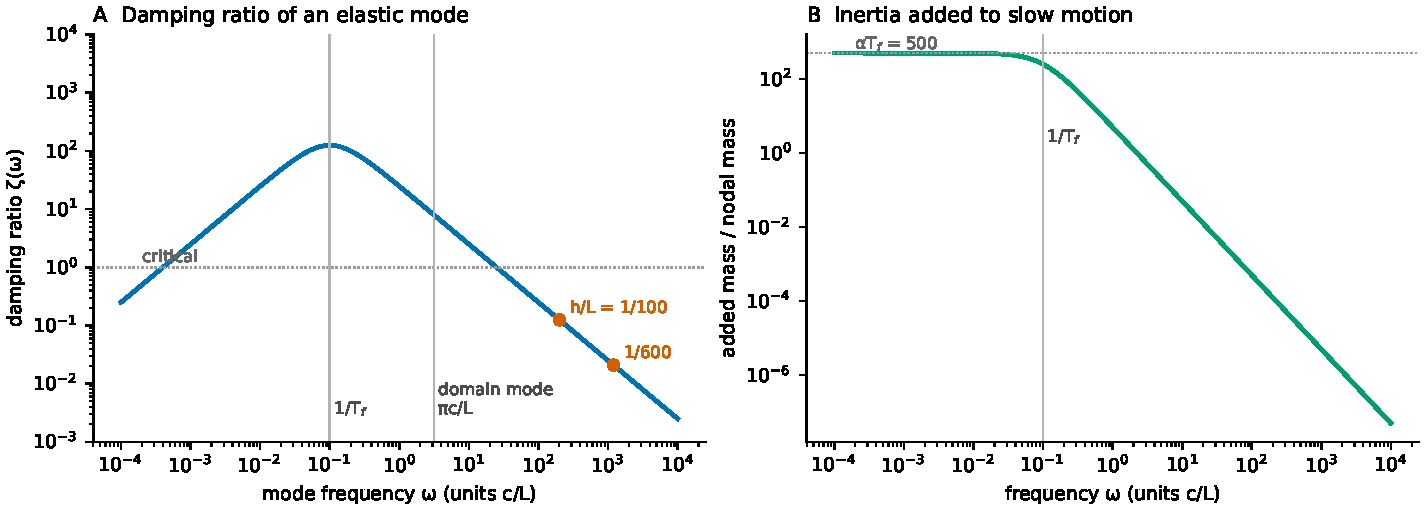
\includegraphics[width=\textwidth]{hp_response.pdf}
  \caption{Frequency response of the high-pass damping with the default parameters
  ($\alpha=50\,c/L$, $T_f=10\,L/c$); frequencies in units of $c/L$.
  \textbf{A}: damping ratio $\zeta(\omega)$ of an elastic mode. The force vanishes for steady
  motion (left), peaks near the cutoff $1/T_f$, overdamps the slowest domain mode ($\pi c/L$,
  $\zeta\approx8$), and damps mesh-scale modes ($\omega_h\approx2c/h$, orange dots for $h/L=1/100$
  and $1/600$) weakly per oscillation but strongly per time step. \textbf{B}: the inertia the
  force adds to slow motion: $\alpha T_f=500$ times the nodal mass below the cutoff, vanishing above
  it.}
  \label{fig:hp}
\end{figure}

%======================================================================
\section{Strain-rate averaging for the creep law}
\label{sec:avg}

\subsection{Formulation}
With \code{control.is\_using\_mixed\_visc\_strain\_rate = yes}, before the stress update each step:
\begin{enumerate}
\item every element $e$ contributes $V_e\,\edot^{(e)}$, its volume times its own strain-rate
  invariant;
\item every node $n$ takes the volume-weighted mean over its support patch,
  $\bar I_n=\sum_{e\ni n}V_e\edot^{(e)}/\sum_{e\ni n}V_e$;
\item every element takes the mean of its nodes, $\edot^{*(e)}=\frac1{N}\sum_{n\in e}\bar I_n$
  ($N=3$ in 2D, 4 in 3D).
\end{enumerate}
The creep viscosity is evaluated as $\eta_e=\eta(\edot^{*(e)},T_e,\dots)$, with the usual
\code{min\_strain\_rate} floor. The stress update itself, the elastic and plastic parts and the
plastic flow still use each element's own strain-rate tensor. The averaged invariant is
recomputed from the current strain rate every call, so it never lags.

This is exactly the round trip that DES already applies for the nodal mixed discretization (NMD):
\code{compute\_dvoldt}/\code{compute\_edvoldt} average the volumetric strain rate and
\code{NMD\_stress} the pressure increment, to avoid volumetric locking of linear triangles. Here
the same operator is applied to the scalar the creep law reads. Mathematically it is a lumped
$L^2$ projection of the piecewise-constant field onto continuous piecewise-linear functions and
back, i.e. the simplest form of gradient (patch) recovery, which gives a better pointwise
estimate of the strain rate than the raw element value on linear elements.

Implementation: 9 files, +76/$-$7 lines on branch \code{feat/mixed-visc-strain-rate}; one new
element array; OpenMP-parallel loops; refused on GPU builds. With the option off the code is
bit-for-bit identical to its parent on the 2D and 3D benchmark suites (\code{make cmp}).

\subsection{Properties of the operator}
We measured the operator $A$ directly on the fine rift mesh at 0.6\,Myr (median element size
$h=3.4$\,km in the column, defined as $\sqrt{2\times\text{area}}$):
\begin{itemize}
\item \emph{Conservative}: $\sum_eV_e\edot^{*(e)}=\sum_eV_e\edot^{(e)}$ exactly (measured
  relative change $\sim10^{-18}$), because the nodal weights $\sum_{e\ni n}V_e$ are the full
  patch volumes.
\item \emph{Consistent}: constants are reproduced exactly; a linear field is reproduced to
  $0.04\,h|\nabla f|$ (median); the error on a quadratic is $0.2\,h^2f''$.
\item \emph{Local}: the rms radius of the weights is $0.93\,h$ (3.1\,km); two passes give
  $1.32\,h$, three $1.61\,h$ (Fig.~\ref{fig:kernel}B,C).
\item \emph{Scale-selective}: Fig.~\ref{fig:kernel}A and Table~\ref{tab:gain} give the fraction of
  a sinusoid's amplitude that survives. One pass removes 92\,\% of the $2h$ checkerboard, which a
  linear mesh cannot represent anyway, keeps 92\,\% at $10h$ and 98\,\% at $20h$.
\item \emph{Vanishing on refinement}: the radius scales with $h$, so the model converges to the
  same continuum problem as the mesh is refined.
\end{itemize}

\begin{table}[h]
  \centering\small
  \caption{Amplitude kept by the averaging operator on the fine rift mesh (column, $h=3.4$\,km),
  for sinusoids of wavelength $\lambda$, averaged over six orientations.}
  \label{tab:gain}
  \begin{tabular}{lccccccc}
  \toprule
  $\lambda/h$ & 2 & 3 & 4 & 6 & 10 & 20 & 30\\
  \midrule
  1 pass   & 0.08 & 0.36 & 0.58 & 0.79 & 0.92 & 0.98 & 0.99\\
  2 passes & 0.01 & 0.14 & 0.34 & 0.62 & 0.84 & 0.96 & 0.98\\
  3 passes & 0.00 & 0.06 & 0.20 & 0.49 & 0.78 & 0.94 & 0.97\\
  \bottomrule
  \end{tabular}
\end{table}

\begin{figure}[t]
  \centering
  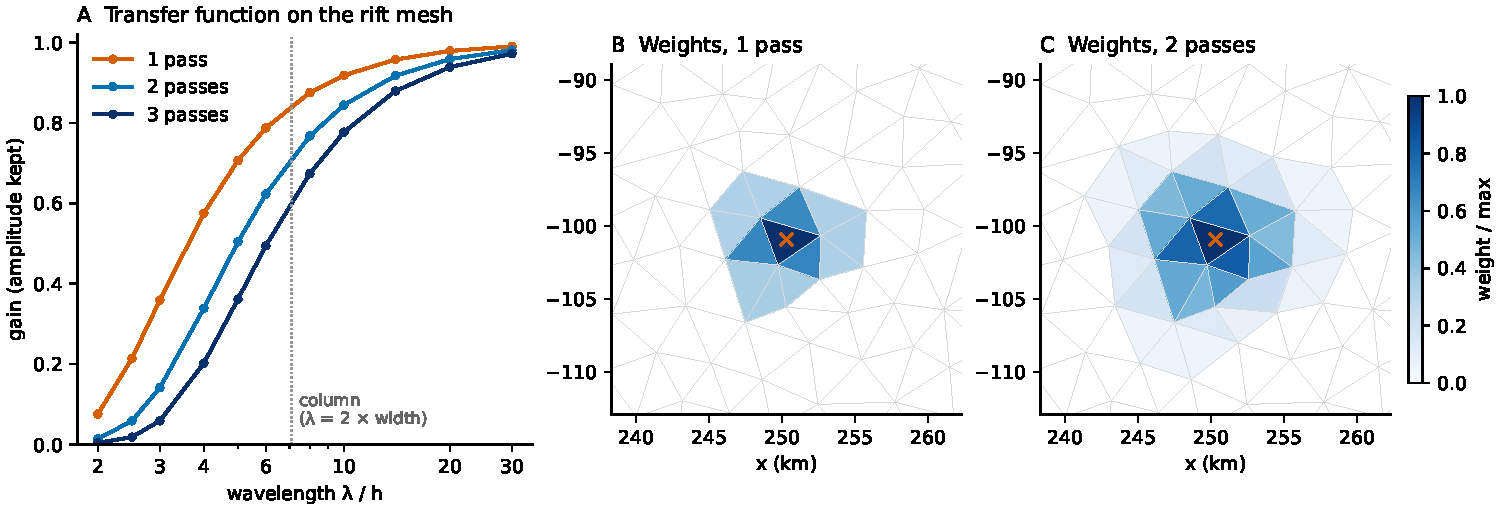
\includegraphics[width=\textwidth]{kernel.pdf}
  \caption{The averaging operator measured on the fine rift mesh at 0.6\,Myr.
  \textbf{A}: transfer function --- the fraction of a sinusoid's amplitude kept, against its
  wavelength in element sizes, for one, two and three passes. The dotted line marks the width of
  the low-viscosity column ($\approx12$\,km $\approx3.5\,h$). \textbf{B, C}: the weights with which
  the surrounding elements enter the averaged strain rate of the element marked by the cross, for
  one pass (the element, its edge and vertex neighbours) and two passes (normalized to the
  largest weight; grey lines are the mesh).}
  \label{fig:kernel}
\end{figure}

\subsection{Why one pass and not two}
The question is what the averaging removes and what it costs. We restarted the damped fine rift
from 0.6\,Myr for 20\,000 steps with 0, 1, 2 and 3 passes (a temporary option, since removed):

\begin{table}[h]
  \centering\small
  \caption{Restart tests from the damped fine rift at 0.6\,Myr, after 20\,000 steps. Speckle: rms
  element anomaly of $\log_{10}$, column/flanks. Profile change: rms difference of the
  cross-rift profile of $\log_{10}\eta$ (6\,km bins, 60--140\,km deep) from the 1-pass run.}
  \label{tab:passes}
  \begin{tabular}{lcccc}
  \toprule
  passes & 0 & 1 & 2 & 3\\
  \midrule
  $\eta$ speckle      & 0.220 / 0.066 & 0.017 / 0.007 & 0.013 / 0.006 & 0.011 / 0.006\\
  $\edot$ speckle     & 0.327 / 0.098 & 0.194 / 0.059 & 0.189 / 0.053 & 0.184 / 0.050\\
  profile change      & 0.052 & --- & 0.031 & 0.054\\
  \bottomrule
  \end{tabular}
\end{table}

One pass removes 92\,\% of the viscosity speckle. A second pass removes almost nothing more ---
the viscosity is already smooth, and the strain-rate speckle that remains is not driven by the
viscosity (Sect.~\ref{sec:restart}) --- but it shifts the large-scale viscosity profile by as much
as switching the averaging off. The reason is visible in Fig.~\ref{fig:kernel}A: the column is
only $\approx3.5\,h$ wide, where a second pass already removes two thirds of the amplitude. One
pass is the smallest operator that removes the $2h$ mode, it is the operator DES already uses for
NMD, and it leaves resolved structure ($\ge10h$) nearly intact. We therefore keep one pass and no
pass-count option.

%======================================================================
\section{Results: core complex}
\label{sec:cc}

\subsection{Research resolution (167\,m), 0--30\,kyr}
The setup is the example core complex with $h=167$\,m and a seed of half-width 1.5\,km and initial
plastic strain 0.1 (\code{cc2-*}). Damping uses the defaults ($\alpha=5\times10^{-8}$\,s$^{-1}$).

\begin{figure}[H]
  \centering
  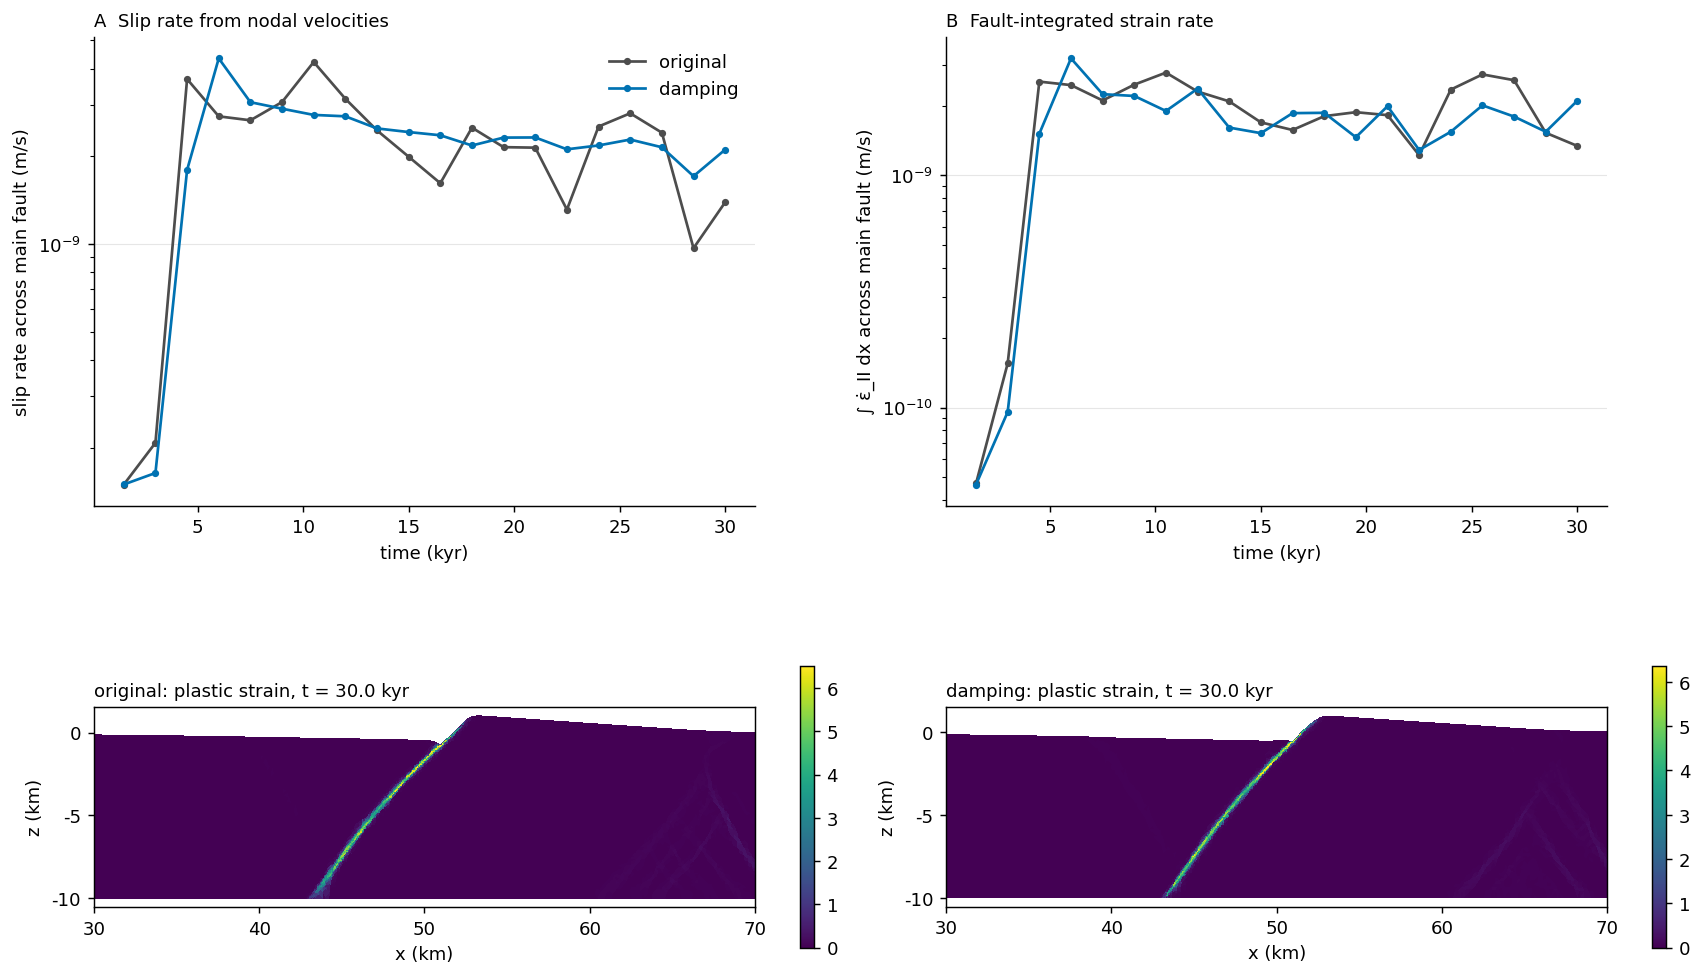
\includegraphics[width=0.95\textwidth]{fig_cc.png}
  \caption{Core complex at 167\,m, original (grey) and damped (blue). \textbf{A}: slip rate across
  the main fault from nodal velocities (mean of $z=3,5,7$\,km). \textbf{B}: $\int\edot\,dx$ across
  the fault. Bottom: plastic strain at 30\,kyr, original (left) and damped (right). The fault
  geometry is the same; the damped slip rate is smooth where the original swings by factors of 2.}
  \label{fig:cc167}
\end{figure}

\begin{figure}[H]
  \centering
  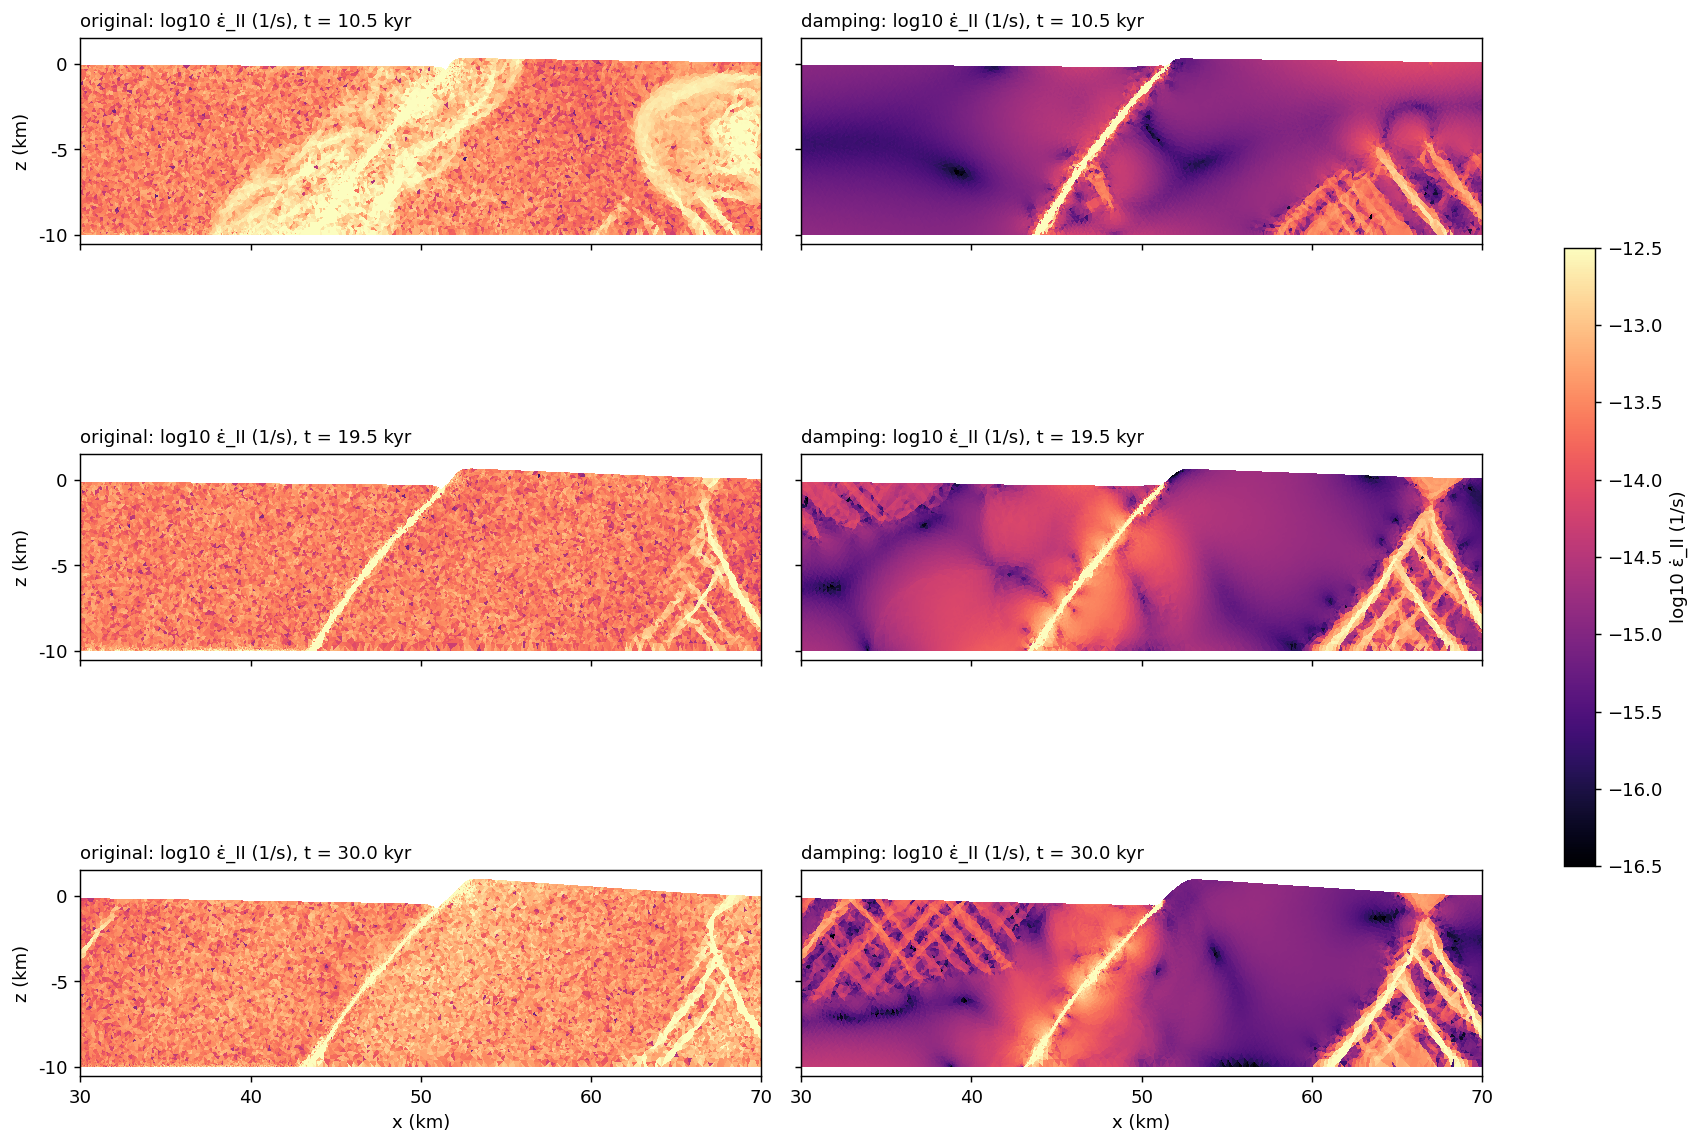
\includegraphics[width=0.95\textwidth]{fig_cc_strainrate.png}
  \caption{$\log_{10}\edot$ at 10.5, 19.5 and 30\,kyr, 167\,m; original (left) and damped (right);
  instantaneous fields. The original's background is uniform element-scale noise at
  $\sim10^{-14}$\,s$^{-1}$ that hides everything but the main fault, and at 10.5\,kyr a broad burst
  around it. In the damped run the background falls to $10^{-15}$--$10^{-16}$\,s$^{-1}$ and
  shows the smooth elastic strain field around the fault, a footwall band, and conjugate
  mesh-scale bands in both hanging wall and footwall that the noise hid in the original.}
  \label{fig:cc167sr}
\end{figure}

Over 15--30\,kyr the slip-rate jump falls from 0.44 to 0.11 and the plastic-integral jump from 0.23
to 0.05; the background p10 drops from $-14.03$ to $-15.61$. The fault position agrees within
0.1\,km at all three depths, and the mean slip rate is $2.19\times10^{-9}$\,m/s damped against
$1.98\times10^{-9}$ original (Table~\ref{tab:conv}): the original's mean is pulled down by its
collapses.

\subsection{Convergence: 1000, 500 and 167\,m}
To judge which run is closer to the converged answer we ran the same setup at 1000 and 500\,m
(Fig.~\ref{fig:conv}, Table~\ref{tab:conv}).

\begin{table}[h]
  \centering\small
  \caption{Core complex (167\,m setup) at three resolutions, original vs damped. Jumps and band
  width over 15--30\,kyr; ``vs ref.'' is the median $|\ln|$ ratio of the slip-rate series to the
  167\,m original.}
  \label{tab:conv}
  \begin{tabular}{lcccccccc}
  \toprule
  run & fault $x$ at 3/5/7\,km & \multicolumn{2}{c}{jump} & \multicolumn{2}{c}{slip (m/s)} & band & bg p10 & vs ref.\\
      & (km) & slip & plastic & 5--15 kyr & 15--30 kyr & (km) & & \\
  \midrule
  orig 1000\,m & 49.1/47.2/44.8 & 0.05 & 0.02 & 2.47e-9 & 2.22e-9 & 1.80 & $-14.70$ & 0.17\\
  damp 1000\,m & 49.6/47.0/44.8 & 0.11 & 0.05 & 2.49e-9 & 2.20e-9 & 1.74 & $-15.72$ & 0.27\\
  orig 500\,m  & 49.7/47.8/45.9 & 0.08 & 0.02 & 2.70e-9 & 2.19e-9 & 1.22 & $-14.82$ & 0.15\\
  damp 500\,m  & 49.6/47.7/45.8 & 0.07 & 0.04 & 2.67e-9 & 2.22e-9 & 1.41 & $-15.64$ & 0.21\\
  orig 167\,m  & 48.7/46.9/45.4 & 0.44 & 0.23 & 3.05e-9 & 1.98e-9 & 0.31 & $-14.03$ & ---\\
  damp 167\,m  & 48.6/46.9/45.4 & 0.11 & 0.05 & 3.05e-9 & 2.19e-9 & 0.28 & $-15.61$ & 0.17\\
  \bottomrule
  \end{tabular}
\end{table}

\begin{figure}[H]
  \centering
  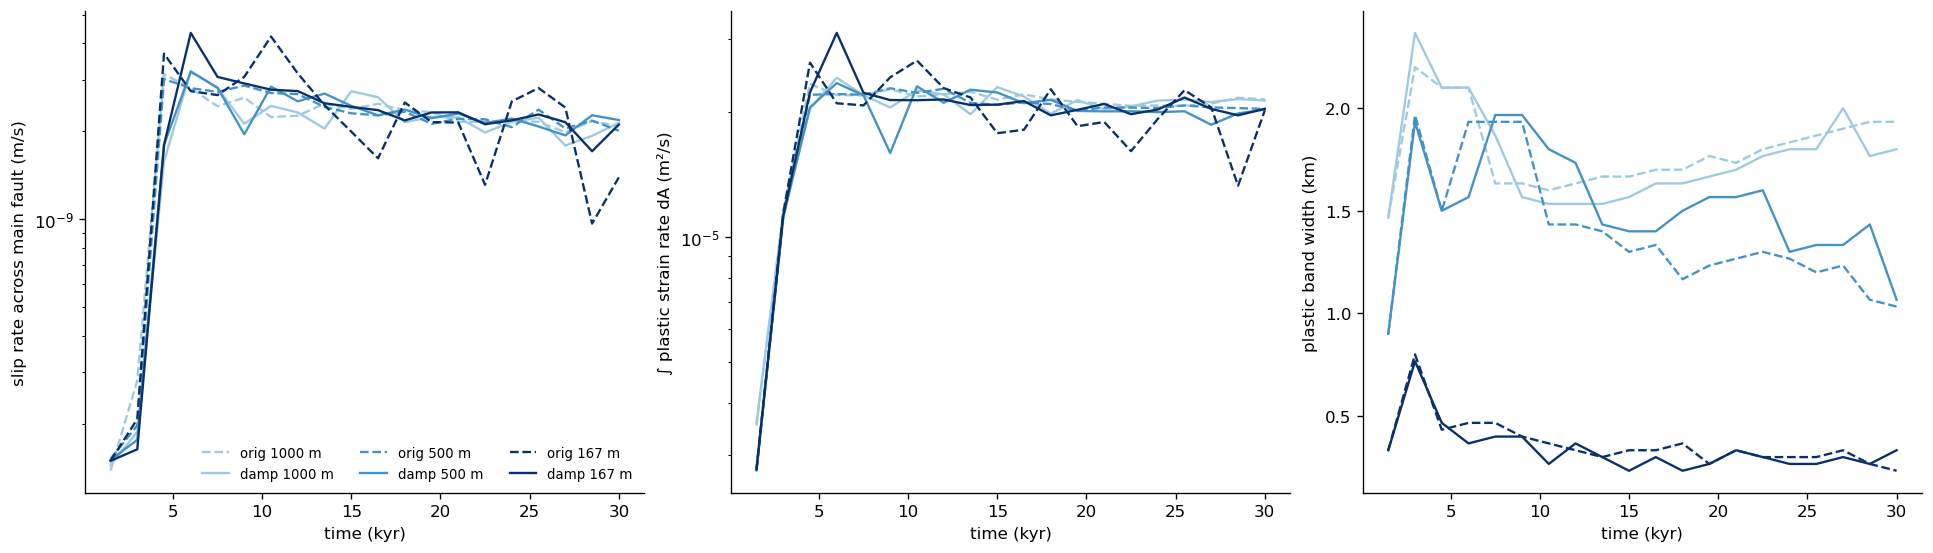
\includegraphics[width=\textwidth]{fig_cc_conv.png}
  \caption{Convergence of the core complex (167\,m setup), 0--30\,kyr. Dashed: original; solid:
  damped; light to dark blue: 1000, 500, 167\,m. Left: slip rate across the main fault. Middle:
  plastic-strain-rate integral. Right: plastic band width. At each resolution the damped run
  follows the original. Slip rate converges to $\approx2.2\times10^{-9}$\,m/s; the only outlier is
  the 167\,m original, whose collapses (e.g. 22.5 and 28.5\,kyr) pull it down. The plastic integral
  agrees within $\approx10$\,\% across resolutions; the band width is set by the mesh (a few
  elements) and does not converge.}
  \label{fig:conv}
\end{figure}

Four conclusions follow. (i) At every resolution the damped run follows the original: same fault
position (within 0.5\,km), same early slip rate, same band width within the scatter. (ii) The slip
rate converges, to $\approx2.2\times10^{-9}$\,m/s; the damped 167\,m run sits on it, the original
167\,m run does not, because of its noise. The plastic integral also converges: every run is within
7--14\,\% (median) of the 167\,m original. (iii) The noise of the plastic integral is cut five-fold
by the damping at 167\,m (0.23$\to$0.05), but at 1000 and 500\,m, where the original is already quiet
(0.02), the damped run is somewhat noisier (0.04--0.05). (iv) The band width (1.8 to 0.3\,km) is
controlled by the element size, not by the damping; it is not a convergent quantity in this model
(Sect.~\ref{sec:lim}).

\subsection{Example resolution (1\,km) to 150\,kyr; choice of $\alpha$ and $T_f$}
The example \code{core-complex.cfg} (seed half-width 1.2\,km, initial plastic strain 0.5,
$h=1$\,km), unchanged except for \code{max\_time\_in\_yr} = 150\,000, was run four ways: original;
damped with the defaults ($\alpha=5\times10^{-8}$, $T_f=10^{10}$\,s); damped with
$\alpha=8.35\times10^{-9}$, which keeps the per-oscillation damping $\zeta_h\propto\alpha h$ of
the 167\,m runs; and damped with $T_f=10^9$\,s, which lowers the added mass $\alpha T_f$ from 500 to
50. A run with damping and strain-rate averaging was bit-identical in its fields to the damped run:
this example is elasto-plastic, has no creep law, and the averaging has nothing to act on.

\begin{table}[h]
  \centering\small
  \caption{Example core complex (1\,km) to 150\,kyr. Per window: slip-rate jump / plastic-integral
  jump / mean slip ($10^{-9}$\,m/s) / band width (km). Bottom: fault position at 150\,kyr and
  median $|\ln|$ ratio to the original of slip rate and plastic integral.}
  \label{tab:cclo}
  \begin{tabular}{lcccc}
  \toprule
  window (kyr) & original & $\alpha$=5e-8, $T_f$=1e10 & $\alpha$=8.35e-9 & $T_f$=1e9\\
  \midrule
  15--45   & 0.10/0.05/1.95/0.51 & 0.31/0.09/1.53/0.57 & 0.30/0.03/1.43/0.46 & 0.28/0.05/1.18/0.81\\
  45--75   & 0.60/0.66/1.93/0.95 & 0.15/0.07/1.84/0.60 & 0.19/0.09/1.54/0.73 & 0.32/0.03/1.51/0.57\\
  75--105  & 0.17/0.11/1.85/1.87 & 0.18/0.06/1.89/1.41 & 0.24/0.09/1.73/1.35 & 0.20/0.09/1.86/0.87\\
  105--150 & 0.43/0.06/1.77/2.66 & 0.18/0.09/1.71/2.01 & 0.40/0.12/1.48/2.03 & 0.38/0.06/1.67/1.98\\
  \midrule
  fault $x$ (km) & 47.3/45.0/43.0 & 47.4/44.8/42.4 & 47.4/44.9/41.1 & 46.8/44.1/41.4\\
  dev. slip / plastic & --- & 0.14 / 0.03 & 0.26 / 0.03 & 0.30 / 0.03\\
  bg p10 (105--150) & $-14.55$ & $-15.81$ & $-15.42$ & $-15.65$\\
  \bottomrule
  \end{tabular}
\end{table}

\begin{figure}[H]
  \centering
  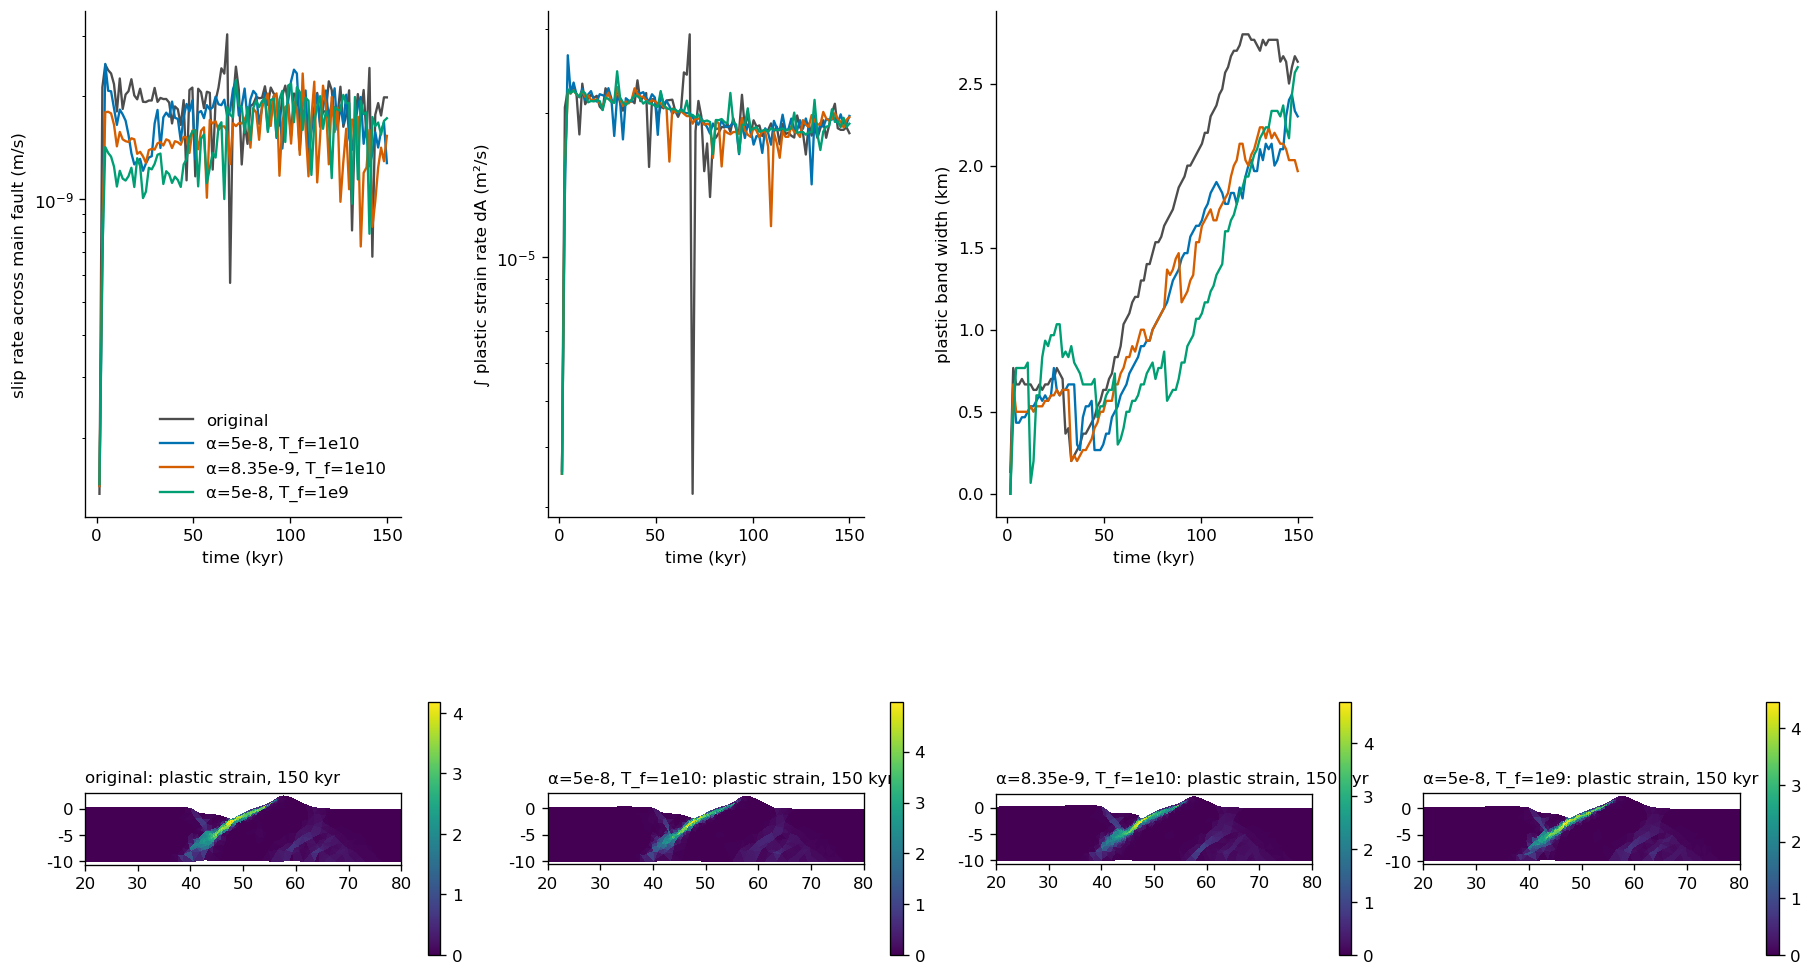
\includegraphics[width=\textwidth]{fig_cc_lo_tf9.png}
  \caption{Example core complex at 1\,km to 150\,kyr. Grey: original; blue: default damping;
  orange: $\alpha=8.35\times10^{-9}$; green: $T_f=10^9$\,s. Top, left to right: slip rate across
  the main fault, plastic-strain-rate integral, plastic band width. The original collapses at
  69\,kyr (slip $\div3$, sharp drop of the plastic integral) and again at 132 and 142\,kyr; no
  damped run does. The plastic integrals of all four runs agree within 3\,\% (median). Bottom: plastic strain at 150\,kyr for the original and the three damped runs (colour
  scales differ: maximum $\approx4.2$ original, $\approx5$ damped).}
  \label{fig:cclo}
\end{figure}

\begin{figure}[p]
  \centering
  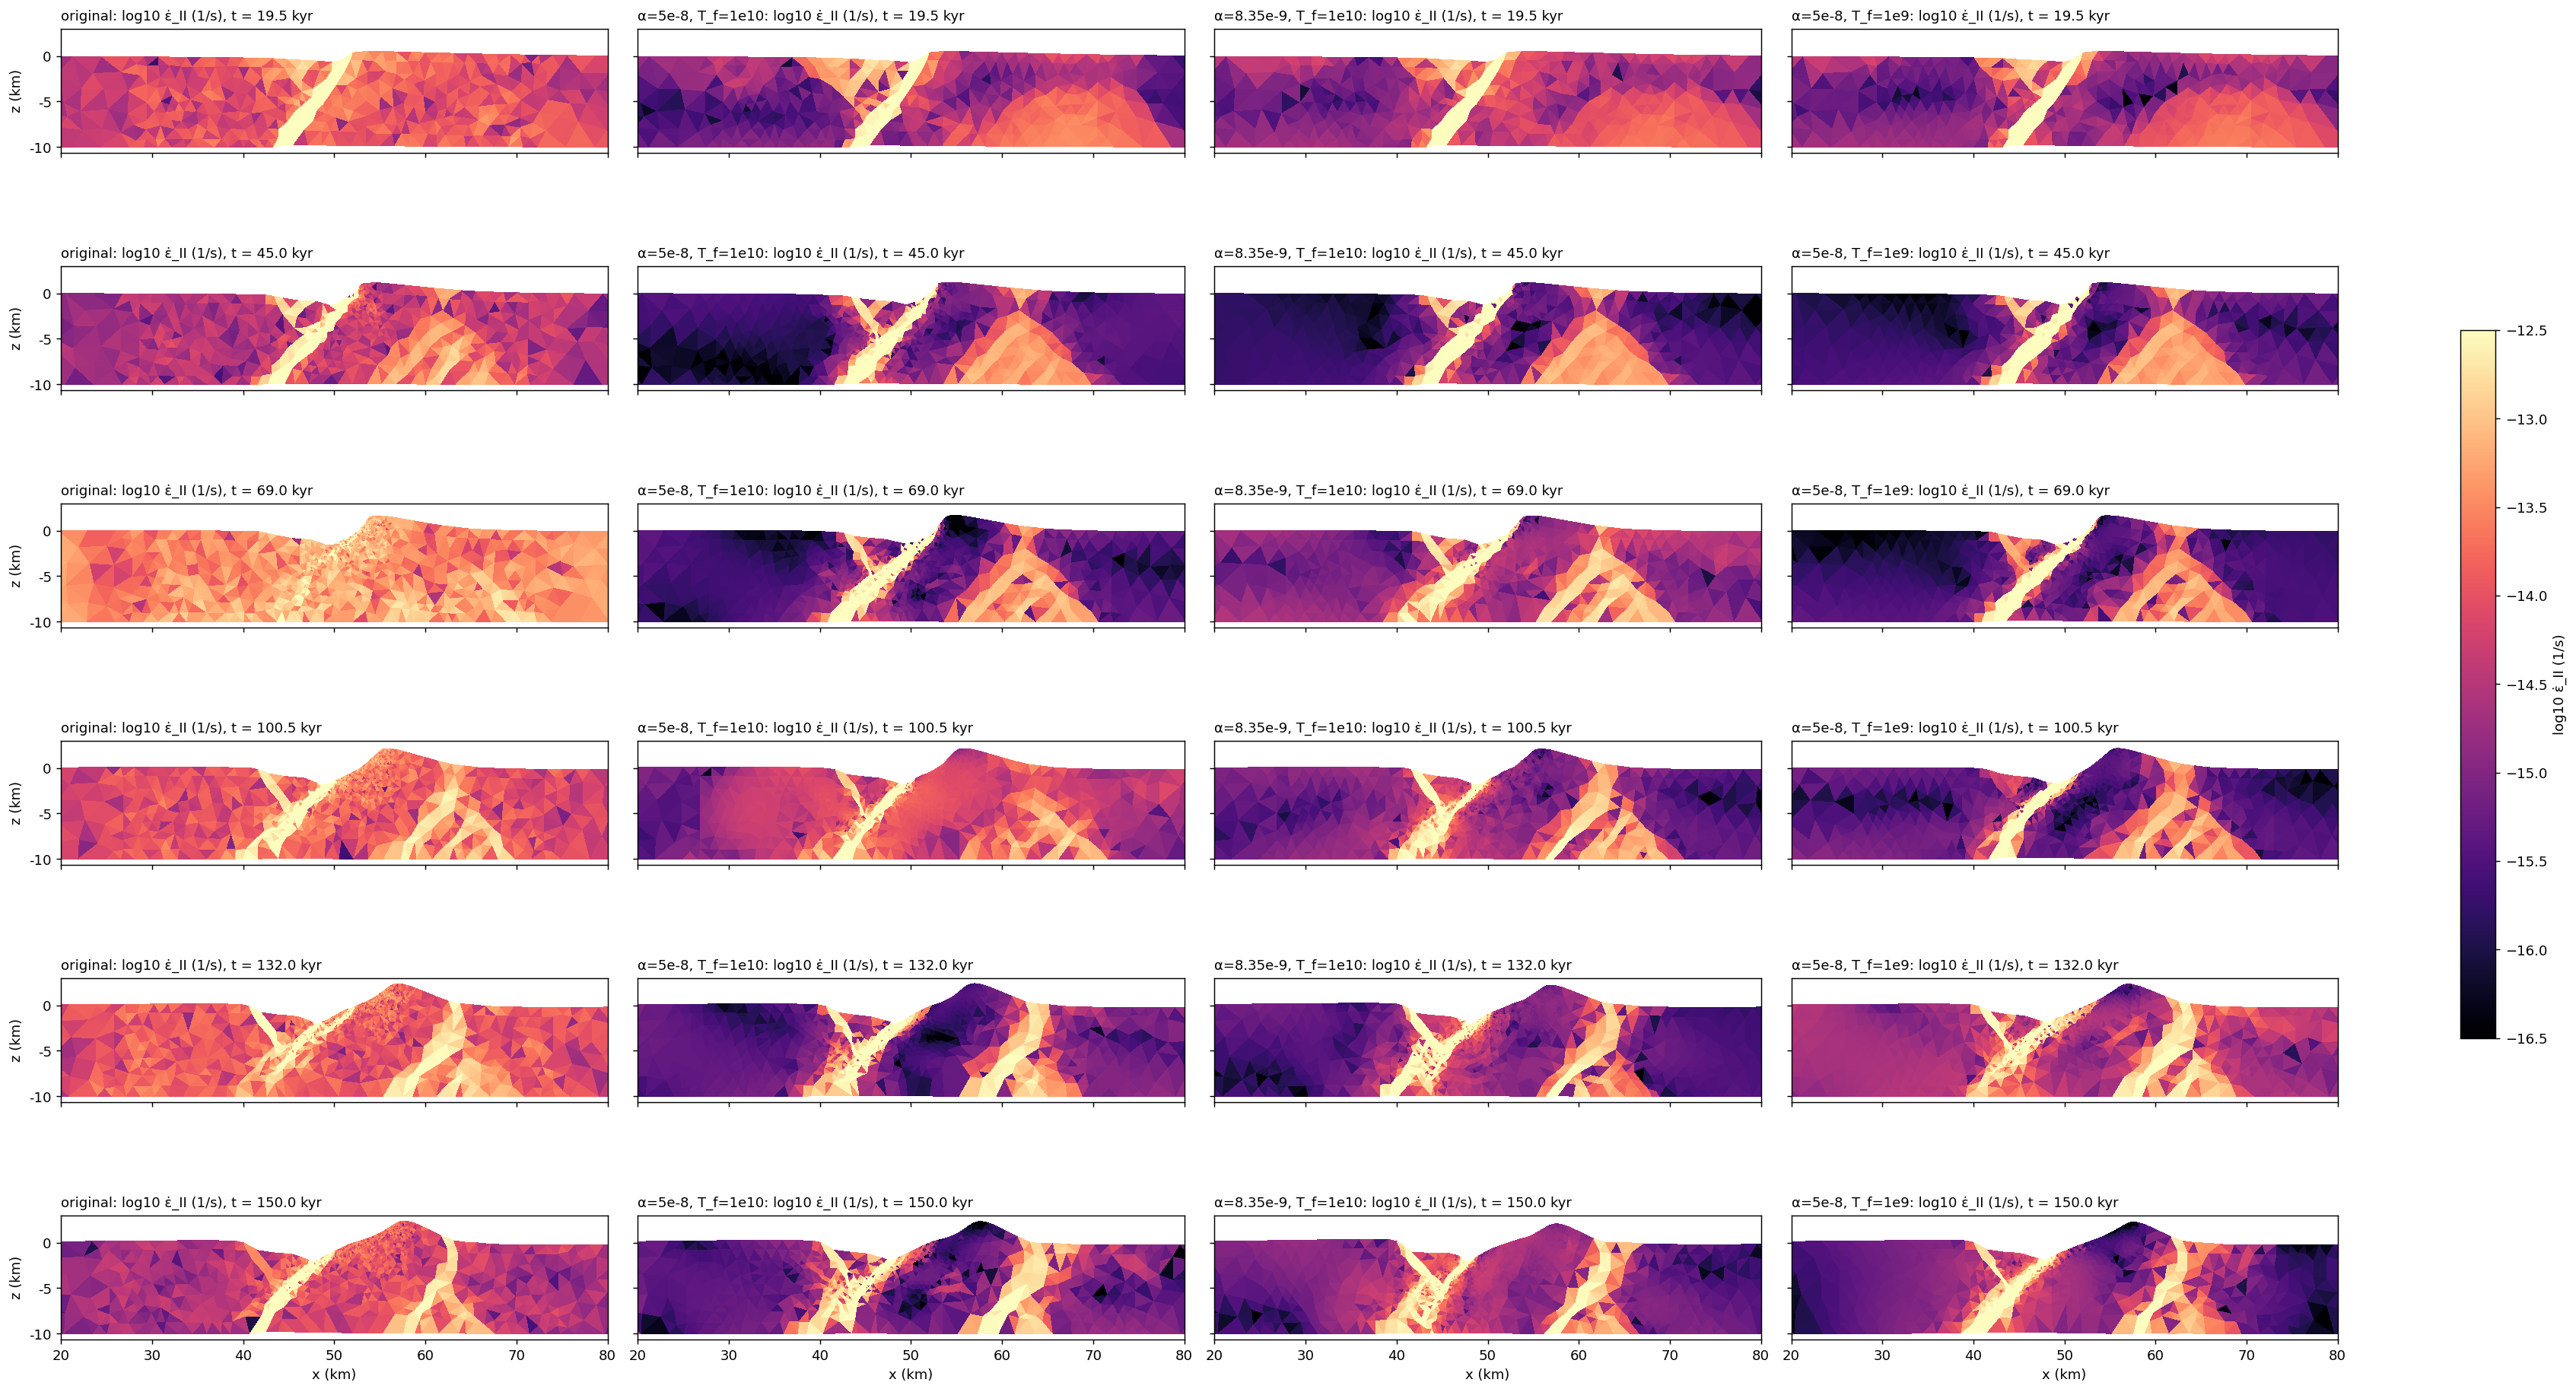
\includegraphics[width=\textwidth]{fig_cc_lo_tf9_strainrate.png}
  \caption{$\log_{10}\edot$ for the runs of Fig.~\ref{fig:cclo} at 19.5, 45, 69, 100.5, 132 and
  150\,kyr (rows); columns: original, default damping, $\alpha=8.35\times10^{-9}$,
  $T_f=10^9$\,s. All damped runs lower the background by about an order of magnitude and keep the
  main detachment, its conjugates at 40--45\,km and the footwall band reaching the surface at
  $\approx62$\,km. At 69\,kyr the original has lost the localized fault altogether; the damped runs
  have not. With the default damping the dome shows frozen very slow elements at 132--150\,kyr, the
  detachment is fragmented near 40--45\,km at 150\,kyr, and a straight-edged block of uniform
  strain rate appears at 100\,kyr at $x\approx27$--40\,km (probably a remeshing imprint; not
  investigated). With the smaller $\alpha$ these artefacts are absent and the detachment is
  continuous.}
  \label{fig:cclosr}
\end{figure}

Reading Table~\ref{tab:cclo} and Figs.~\ref{fig:cclo}--\ref{fig:cclosr}:
\begin{itemize}
\item All damped runs keep the original's structure: one detachment dipping beneath the dome at
  $\approx57$\,km, the same conjugates, fault position within 1.9\,km at 7\,km depth and 0.9\,km
  above. None has the original's collapses.
\item The default damping gives the quietest time series after 45\,kyr (slip jump 0.15--0.18
  against 0.17--0.60). Lowering $\alpha$ six-fold or the added mass ten-fold makes the slip rate
  almost as noisy as the original's again, without bringing its mean closer. The plastic integral
  of every damped run stays within 3\,\% (median) of the original's.
\item The smaller $\alpha$ gives the cleanest strain-rate maps (no frozen elements), at the cost of
  that noisier slip rate.
\item Two differences from the original are \emph{independent} of $\alpha$ and $T_f$: slower slip
  between 15 and 45\,kyr ($1.2$--$1.5$ against $1.95\times10^{-9}$\,m/s) and a narrower band late in
  the run (2.0 against 2.7\,km). Since they do not change with a six-fold change of $\alpha$ or a
  ten-fold change of the added mass, they are not caused by the strength of the damping or by its
  inertia. In the 167\,m setup at the same 1\,km resolution the damped and original early slip are
  identical (Table~\ref{tab:conv}), so it is not a general effect of damping either. The most likely
  explanation is path dependence: in this example both runs reorganize at $\approx30$\,kyr (the
  band width collapses in Fig.~\ref{fig:cclo}), and which band takes over is sensitive to small
  differences. This is a hypothesis, not a demonstrated result.
\end{itemize}

\paragraph{Recommendation for $\alpha$ and $T_f$.} Keep the defaults $\alpha=50\,c/L$,
$T_f=10\,L/c$. They depend on the domain and the loading, not on the mesh, so they need no
re-tuning with resolution; the added mass they imply ($\sqrt{500}\approx22$) is far inside the
quasi-static limit; and over the range we tested they give the quietest slip rate without moving
the fault or the converged slip rate. Judge any change by convergent quantities (slip rate, plastic
integral, fault position), not by band width. Lower $\alpha$ only to clean up strain-rate
maps at coarse resolution, accepting a noisier slip rate.

%======================================================================
\section{Results: rifting}
\label{sec:rift}

The rift example (\code{rifting-2d.cfg}/\code{.poly}; elasto-visco-plastic, two materials, power-law
creep with $n=3.05$, $V=\pm10^{-9}$\,m/s) was run to 1\,Myr on the example mesh (resolution 6\,km,
region area limit $4\times10^7$\,m$^2$) and on a finer mesh (region area limit $10^7$\,m$^2$,
6487 initial elements). Damping uses the defaults ($\alpha=10^{-8}$\,s$^{-1}$, $T_f=5\times10^{10}$\,s).
Strain-rate maps are 1000-step averages (Sect.~\ref{sec:problem}).

\subsection{Example mesh}
\begin{table}[h]
  \centering\small
  \caption{Rift on the example mesh, $t>0.2$\,Myr. Deviation: median $|\ln|$ ratio of the plastic
  integral to the original.}
  \label{tab:riftlo}
  \begin{tabular}{lccccc}
  \toprule
  run & jump plastic & jump $\int\edot$ & bg p10 & visc.\ roughness & deviation\\
  \midrule
  original            & 0.034 & 0.365 & $-16.15$ & 0.199 & ---\\
  damping             & 0.014 & 0.088 & $-16.13$ & 0.179 & 1.7\,\%\\
  damping + averaging & 0.018 & 0.063 & $-16.18$ & 0.122 & 0.9\,\%\\
  \bottomrule
  \end{tabular}
\end{table}

\begin{figure}[p]
  \centering
  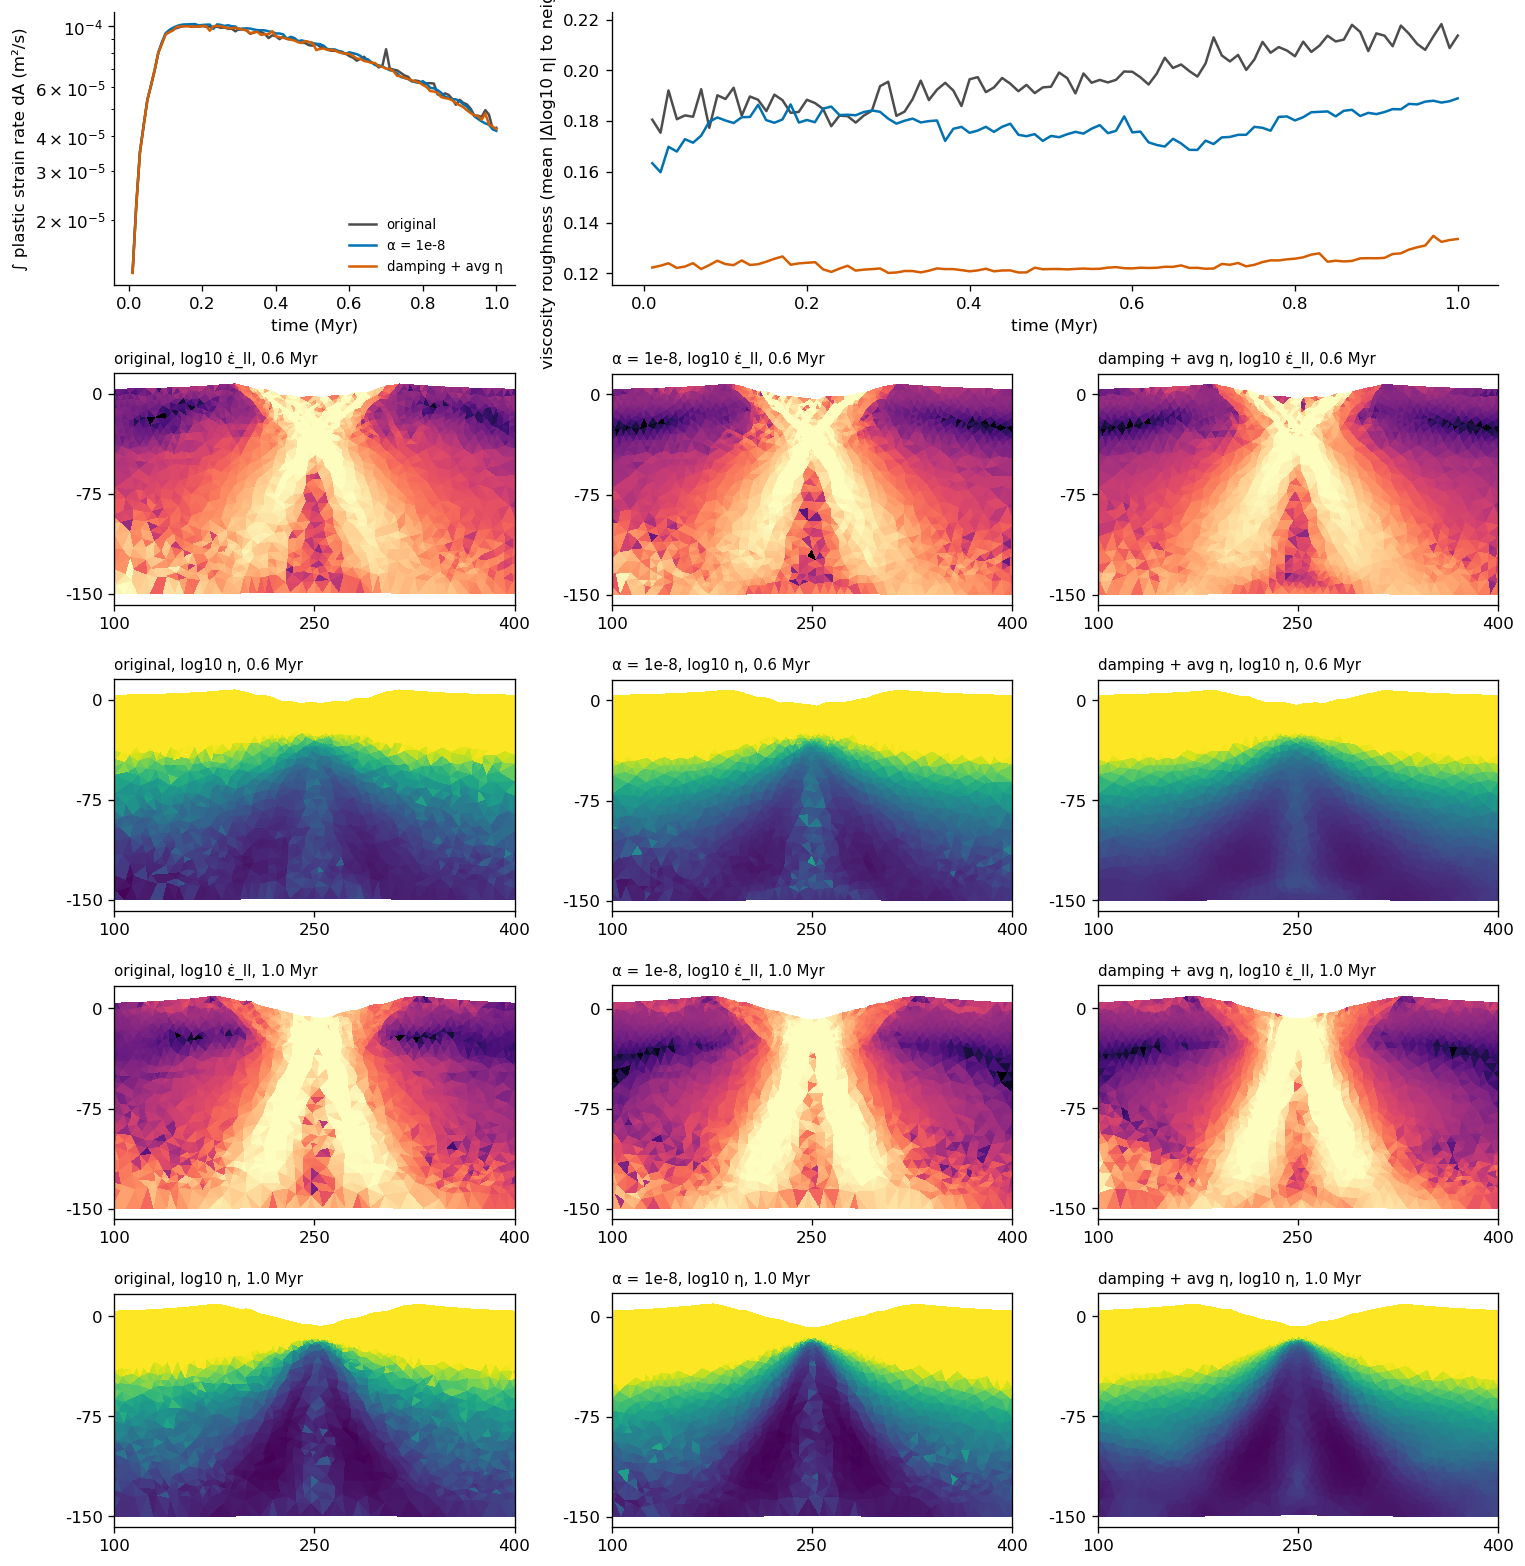
\includegraphics[width=\textwidth]{fig_rift_lo_mv.png}
  \caption{Rift on the example mesh to 1\,Myr. Columns: original, damping ($\alpha=10^{-8}$),
  damping + strain-rate averaging. Top left: plastic-strain-rate integral --- the three curves
  coincide, except for the original's spike at 0.70\,Myr. Top right: viscosity roughness ---
  damping alone lowers it slightly (0.20$\to$0.18), averaging removes most of it (0.12). Rows 2--5:
  $\log_{10}\edot$ (colour $-17$ to $-13.5$) and $\log_{10}\eta$ (19 to 24) at 0.6 and 1.0\,Myr,
  $x=100$--400\,km, depth 0--150\,km. Necking width, the X-shaped shallow shear bands and the
  upwelling column are the same in all three. On this coarse mesh part of the remaining roughness
  is real: the temperature gradient changes $\eta$ appreciably from one 6\,km element to the next.}
  \label{fig:riftlo}
\end{figure}

\subsection{Fine mesh}
\begin{table}[h]
  \centering\small
  \caption{Fine-mesh rift, $t>0.2$\,Myr, including the $\alpha$ scan. Wall time on 4 threads.}
  \label{tab:riftfine}
  \begin{tabular}{lcccccc}
  \toprule
  run & jump plastic & jump $\int\edot$ & bg p10 & visc.\ roughness & deviation & wall (s)\\
  \midrule
  original                          & 0.032 & 0.057 & $-15.93$ & 0.154 & ---   & 6194\\
  damping, $\alpha=1.3\times10^{-9}$ & 0.013 & 0.025 & $-15.90$ & 0.097 & 3.4\,\% & 5838\\
  damping, $\alpha=10^{-8}$ (default)& 0.021 & 0.041 & $-15.89$ & 0.096 & 3.6\,\% & 6017\\
  damping, $\alpha=7.7\times10^{-8}$ & 0.014 & 0.089 & $-15.90$ & 0.103 & 4.2\,\% & 5932\\
  damping + averaging                & 0.015 & 0.021 & $-15.90$ & 0.068 & 2.9\,\% & 5856\\
  \bottomrule
  \end{tabular}
\end{table}

\begin{figure}[p]
  \centering
  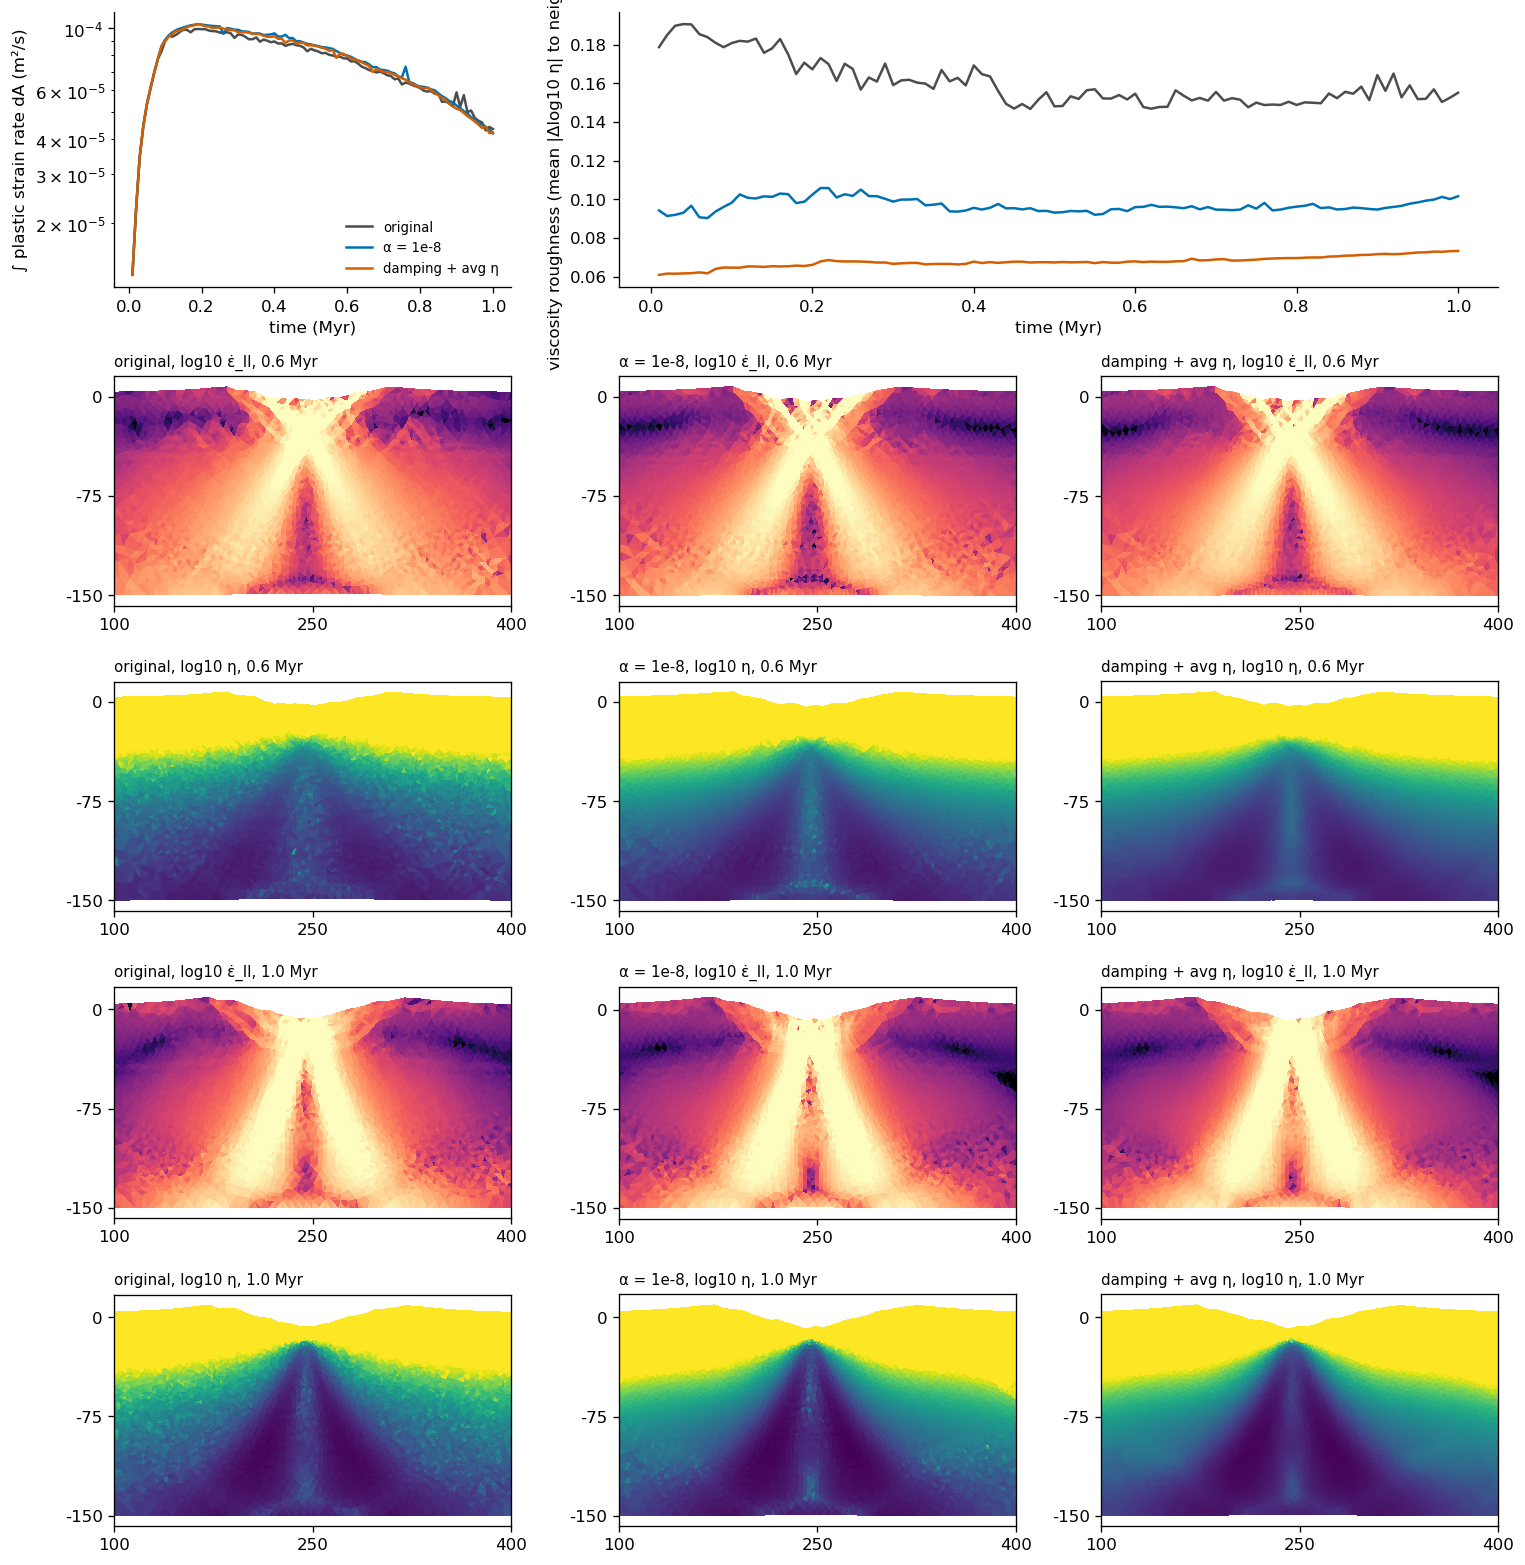
\includegraphics[width=\textwidth]{fig_rift_mv.png}
  \caption{Fine-mesh rift to 1\,Myr; layout as Fig.~\ref{fig:riftlo}. Columns: original, damping,
  damping + averaging. Viscosity roughness: 0.15 original, 0.10 damped, 0.07 with averaging, flat in
  time. The viscosity maps show the progression most clearly: speckle everywhere below the
  lithosphere in the original; speckle left in the flanks and the deep column with damping; a smooth
  field with a sharply outlined low-viscosity wedge and column with averaging. In the strain rate a
  checkerboard persists in the deep column ($z<-75$\,km) even with averaging
  (Sect.~\ref{sec:restart}).}
  \label{fig:riftfine}
\end{figure}

\begin{figure}[p]
  \centering
  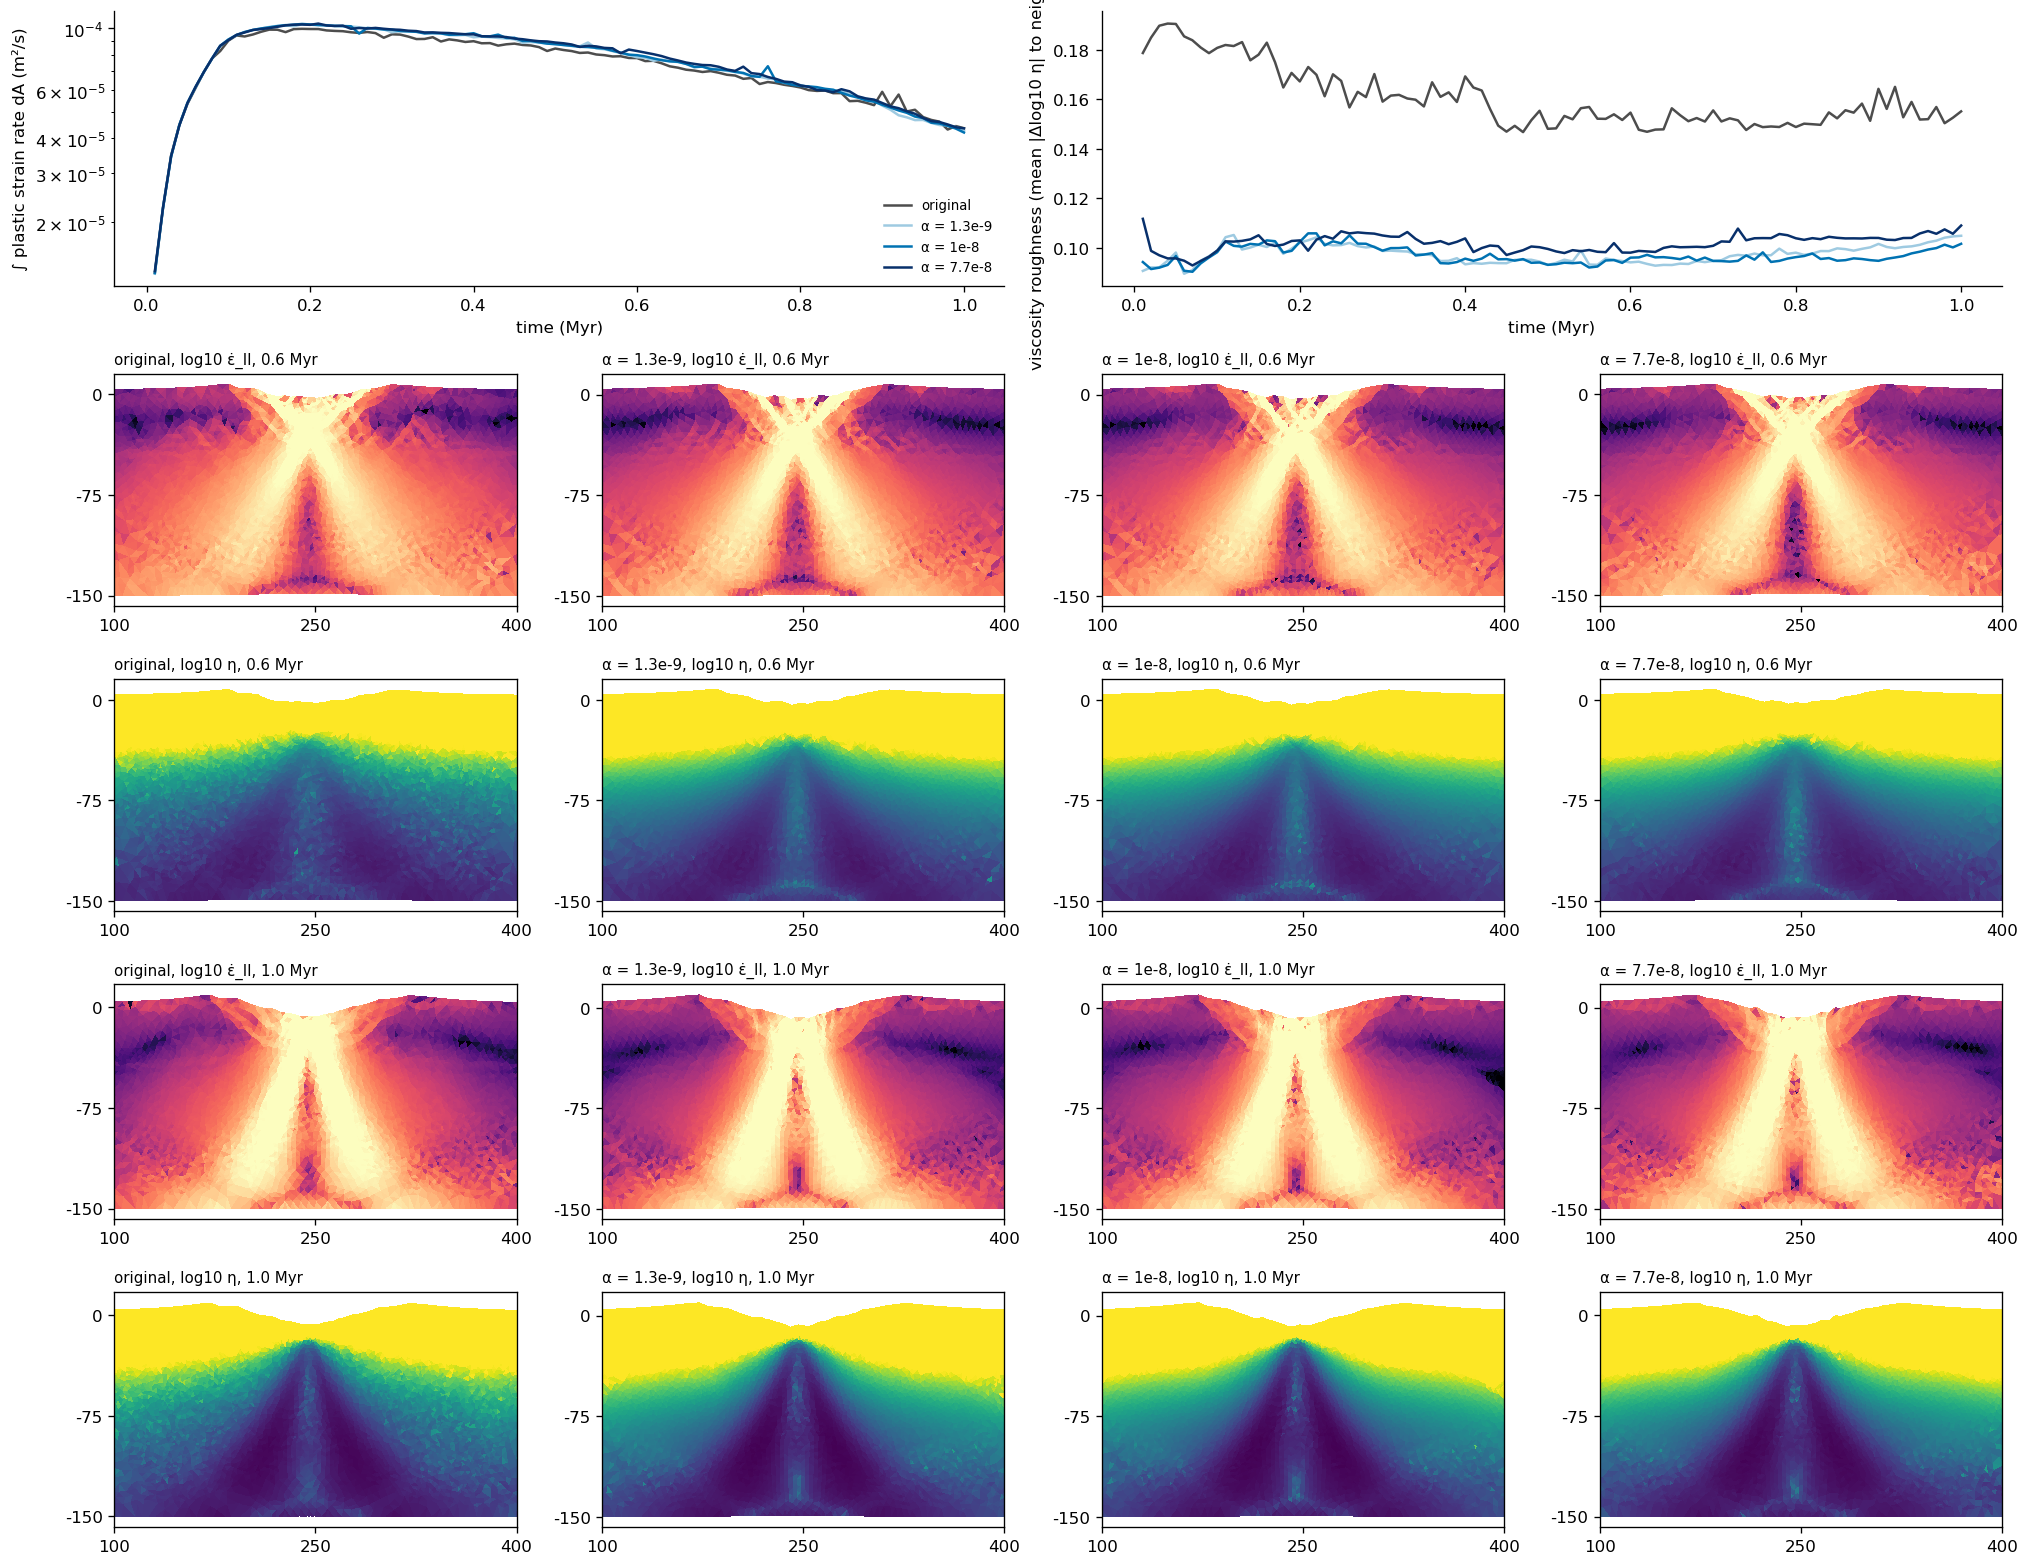
\includegraphics[width=\textwidth]{fig_rift_alpha.png}
  \caption{Fine-mesh rift: sensitivity to $\alpha$ over a factor of 60. Columns: original,
  $\alpha=1.3\times10^{-9}$, $10^{-8}$ (default), $7.7\times10^{-8}$; layout as
  Fig.~\ref{fig:riftlo}. All damped runs give the same plastic integral, the same roughness
  (0.096--0.103) and indistinguishable maps.}
  \label{fig:alpha}
\end{figure}

On both meshes the long-term rift is unchanged: the plastic-integral curve follows the original
within a few per cent over 1\,Myr, minus the original's spikes, and the geometry is the same.
The damping removes most of the time-series noise; the averaging removes most of the viscosity
speckle and lowers the strain-rate-integral jump further (by 30\,\% on the example mesh, 50\,\% on the fine one). With averaging the run is closer to the
original than with damping alone (deviation 0.9 vs 1.7\,\% coarse, 2.9 vs 3.6\,\% fine). The rift is
insensitive to $\alpha$ over a factor of 60.

%======================================================================
\section{What the speckle is: restart tests}
\label{sec:restart}

The fine rift's low-viscosity column ($x\approx240$--252\,km, 60--140\,km deep,
$\eta=10^{20}$--$10^{21}$\,Pa\,s) is speckled 3--5 times more than its flanks. It is not at the
viscosity floor ($10^{19}$; no element there) and not yielding. We restarted the fine runs at
0.6\,Myr with output averaging off to find out what the speckle is (Fig.~\ref{fig:restart}).

\paragraph{Test 1: temporal or frozen?} Outputs every 20 steps for 400 steps. In the original the
column pattern decorrelates within 20 steps (correlation $-0.05$; 51\,\% of elements change sign of
anomaly every 20 steps): it is wave noise, oscillating in time. In the damped run the correlation is
1.000 and no element changes sign: the pattern is frozen. The damping has removed the waves, but a
static element-scale pattern remains, with an amplitude (0.32 in $\log\edot$) similar to the
original's instantaneous noise. Note that in the 1000-step averaged output the original's temporal
noise is partly averaged away while the damped run's frozen pattern is not; this is why damping
alone looks less effective in the viscous part of the rift than in its plastic part.

\paragraph{Test 2: is it the power law?} Same restart, 20\,000 steps, with the creep law replaced
by a Newtonian one matched at $\edot=1.09\times10^{-15}$\,s$^{-1}$ ($A=5.39\times10^{-11}$,
$E=123$\,kJ/mol). Damped, the column strain-rate speckle falls from 0.29 at the restart to 0.046 within 2000
steps, the viscosity speckle to 0.003. Without damping it stays at 0.12--0.19 (wave noise). So the
frozen pattern needs both: the damping removes the waves, the power law sustains the static pattern
by feeding it back through the viscosity.

\paragraph{Test 3: averaging.} With the averaged strain rate in the creep law (damped), the
viscosity speckle falls from 0.22 to 0.017 and the strain-rate speckle from 0.32 to 0.19 (flanks
0.10$\to$0.06). Two passes give 0.189, three 0.184 (Table~\ref{tab:passes}).

\begin{figure}[t]
  \centering
  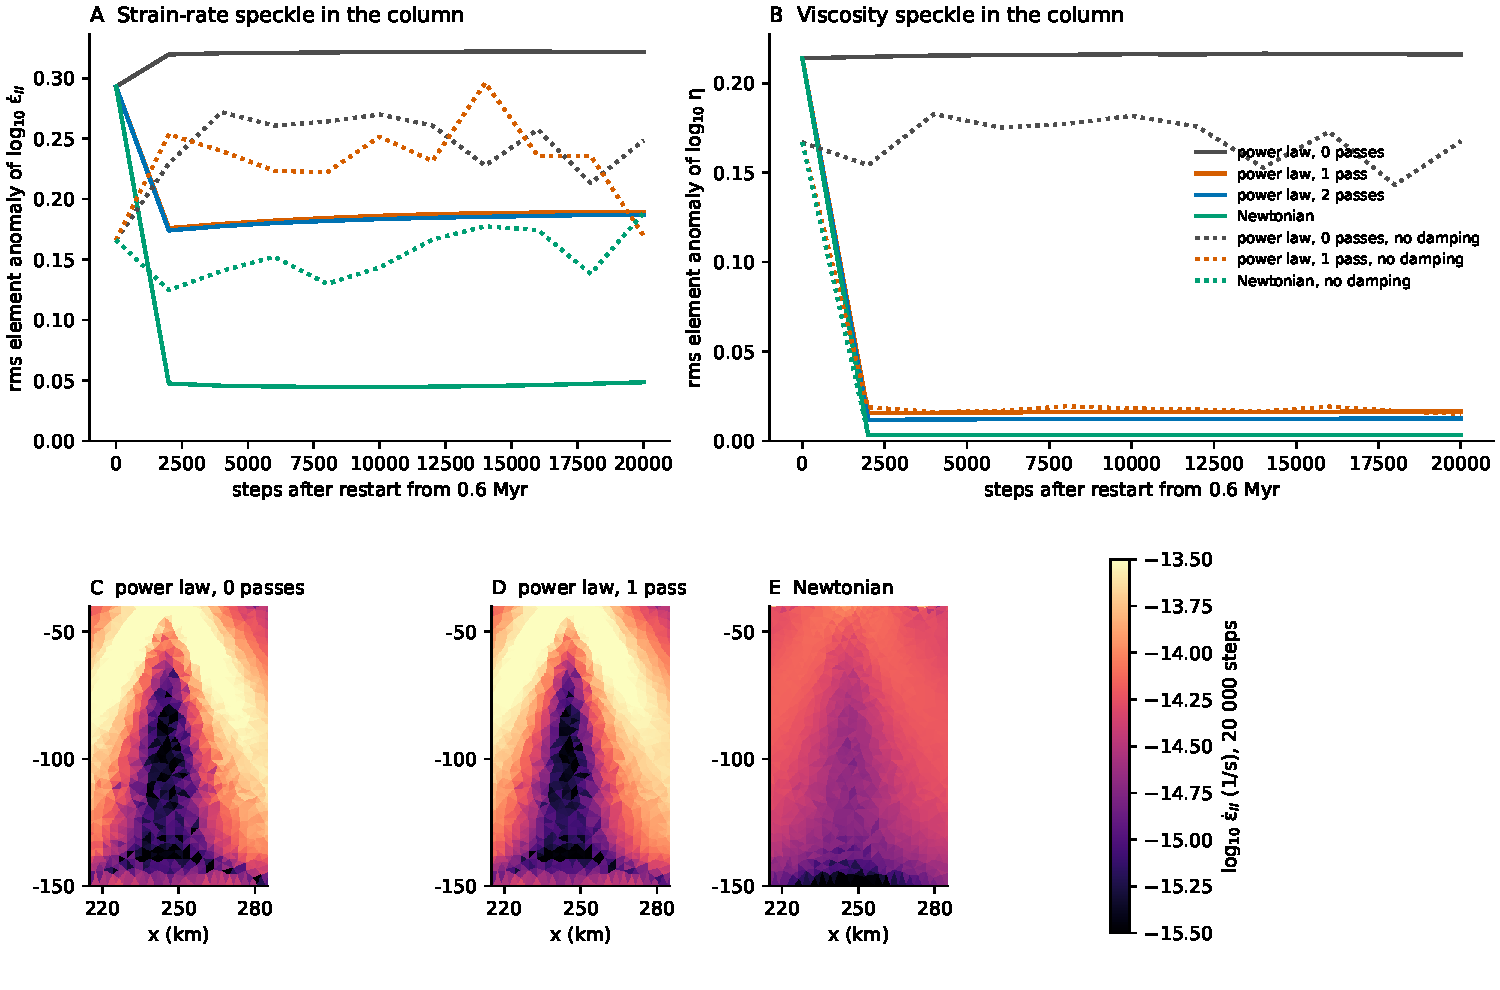
\includegraphics[width=\textwidth]{restart.pdf}
  \caption{Restart tests from the fine rift at 0.6\,Myr (output averaging off; output every 2000
  steps). \textbf{A}: rms element anomaly of $\log_{10}\edot$ in the column against steps. Solid:
  damped; dotted: undamped. Grey: power law; orange: power law with one averaging pass; blue: two
  passes; green: Newtonian. \textbf{B}: the same for $\log_{10}\eta$. \textbf{C--E}:
  $\log_{10}\edot$ around the column after 20\,000 steps (damped) for the power law, the power law
  with averaging, and the Newtonian law. Note that the Newtonian law also changes the large-scale
  flow: the column is a strain-rate minimum on the axis of the upwelling in the power-law runs, much
  less so in the Newtonian one.}
  \label{fig:restart}
\end{figure}

\paragraph{What remains.} After one averaging pass the viscosity is smooth, yet the column
strain-rate speckle settles at 0.19 instead of the Newtonian 0.05, and more passes do not change
it. The remaining checkerboard is therefore not fed by the viscosity. Two observations bear on it
but do not settle it: the column is a local strain-rate minimum on the axis of the upwelling
(median $1.3\times10^{-15}$\,s$^{-1}$ against $2.5\times10^{-15}$ in the Newtonian run), where a
fixed absolute roughness is a larger relative one; and the absolute roughness is also about three
times the Newtonian one ($8.9\times10^{-16}$ against $2.7\times10^{-16}$\,s$^{-1}$). The Newtonian
test changes the large-scale flow and is not a clean control. We have not identified the cause.

%======================================================================
\section{Limitations}
\label{sec:lim}

\paragraph{No length scale; band width stays mesh-dependent.} Neither method introduces a physical
length. The damping acts on time scales only; the averaging has a radius proportional to $h$ and
acts only on the creep viscosity, not on plasticity. Shear bands in the strain-softening
Mohr--Coulomb material therefore remain a few elements wide whatever the damping:
Table~\ref{tab:conv} shows the band narrowing from 1.8 to 0.3\,km as $h$ goes from 1\,km to
167\,m, original and damped alike, while the integrated plastic rate stays within $\approx10$\,\%:
the same deformation is concentrated in a narrower band. This is a property of the
rate-independent, softening plasticity, not of the damping.

\paragraph{A length scale through Duvaut--Lions regularization.} A physical band width can be
introduced by regularizing the plastic flow itself. Branch \code{feat/regularization} implements
the Duvaut--Lions viscoplastic regularization (\code{control.has\_duvaut\_lions},
\code{mat.relaxation\_time} $=\tau$) for the elasto-plastic and elasto-visco-plastic rheologies.
Each step the stress becomes
\begin{equation}
  \boldsymbol\sigma = (1-w)\,\boldsymbol\sigma^{\rm trial} + w\,\boldsymbol\sigma^{\rm return},
  \qquad w = \frac{\Delta t}{\tau+\Delta t},
\end{equation}
a weighted mean of the elastic trial stress and the rate-independent return-mapped stress, and the
plastic-strain increment is scaled by $w$. The overstress above the yield surface relaxes over
$\tau$ instead of instantly; $\tau=\eta_{vp}/G$ corresponds to a viscoplastic viscosity
$\eta_{vp}$. Because the stress may now exceed the yield surface at a rate-dependent amount, the
softening problem stays well posed, and the band acquires a width set by $\tau$, the loading rate
and the softening, not by the mesh: the branch's help text gives
$W\sim\tau G V/\Delta c$, with $\Delta c$ the cohesion lost by softening, calibrated on
\code{examples/core-complex-dl.cfg}, where $\tau=3.3\times10^8$\,s gives $W\approx1.15$\,km. The band
becomes mesh-independent once about five elements span it (below about three it follows the
mesh), so the mesh must resolve $W/5$ wherever a fault can form; a refined zone around the seed plus
MMG plastic-strain refinement is the recommended setup. $\tau=0$ recovers the rate-independent
return bit for bit.

Duvaut--Lions and high-pass damping address different things and are complementary. The
regularization fixes \emph{where} and \emph{how wide} the deformation localizes; the damping
removes the pseudo-elastic waves that a slipping fault radiates in the mass-scaled solver, which a
regularized band still radiates. The two are compatible: on \code{examples/core-complex-dl.cfg}
($\tau=3.3\times10^8$\,s, adaptive mesh, 50\,kyr) adding the damping leaves the fault position
within 0.3\,km, the band width within 0.03\,km after 15\,kyr and the slip rate within 2\,\%, while it
lowers the background strain rate by about an order of magnitude and removes a slip-rate dip at
42\,kyr that Duvaut--Lions alone still shows (see the companion note on Duvaut--Lions). The same branch also has a nonlocal averaging of the plastic-strain
increment (\code{mat.nonlocal\_option}); it widens the softened zone but, as its help text records,
does not by itself make the active fault mesh-independent on the core-complex example (issue
\#123).

\paragraph{Frozen patterns.} The damping removes oscillations, not static element-scale
patterns: once the waves are gone, an element-scale strain-rate pattern can persist (test 1). In
viscous regions the power law sustains it; the strain-rate averaging removes the viscosity part of
it but not the remaining strain-rate checkerboard (Sect.~\ref{sec:restart}). In the plastic core
complex at 1\,km, the default damping leaves a few frozen very slow elements in the dome late in the
run (Fig.~\ref{fig:cclosr}); a smaller $\alpha$ avoids them at the cost of a noisier slip rate.

\paragraph{Resolution dependence of the damping per oscillation.} With $\alpha$ and $T_f$ fixed by
the domain, the per-oscillation damping of mesh-scale modes scales as $\zeta_h\approx12.5\,h/L$:
six times stronger at 1\,km than at 167\,m. Scaling $\alpha$ to keep $\zeta_h$ constant did not
bring the coarse run closer to the original (Sect.~\ref{sec:cc}); the default is kept, but this
dependence is real.

\paragraph{Added mass.} For motion slower than $T_f$ the damping adds an inertia $\alpha T_f M$ and
slows the pseudo waves by $\sqrt{1+\alpha T_f}$. With the defaults this is a factor 22 against an
inertial scaling of $10^5$, harmless here; raising $\alpha$ or $T_f$ by large factors would erode the
quasi-static assumption.

\paragraph{Path dependence.} In the example core complex the damped runs slip more slowly between
15 and 45\,kyr and end with a narrower band than the original, independently of $\alpha$ and $T_f$
and not in the 167\,m setup. We attribute this to the sensitivity of fault reorganization to small
differences, but have not shown it; a short ensemble with perturbed seeds would test it.

\paragraph{Averaging scope.} The averaging affects only the creep viscosity in
\code{update\_stress}. The initial viscosity, the Maxwell blend at remeshing and the monitor output
still use the element's own strain rate. It does nothing in purely elasto-plastic models.

\paragraph{Unexplained residual strain-rate checkerboard} in the low-viscosity column of the fine
rift, after damping and averaging (Sect.~\ref{sec:restart}).

\paragraph{Platforms.} Both options are CPU-only (OpenMP); GPU (OpenACC) builds refuse them. The
damping requires \code{control.is\_quasi\_static} and is refused with \code{control.has\_PT}.

\paragraph{Output averaging.} The default \code{sim.is\_outputting\_averaged\_fields = yes}
averages strain rates over 1000 steps in the rift. It partly hides temporal noise in undamped runs
and not frozen patterns in damped ones, which biases visual comparisons of strain-rate maps;
comparisons should use the same setting, and the instantaneous field when the question is noise.

%======================================================================
\section{Summary}
\begin{itemize}
\item High-pass mass damping removes the pseudo-elastic wave noise of the mass-scaled solver while
  leaving steady slip and creep undamped. Once the fault is established it cuts the slip-rate jump by a factor 2.5--4 (during early
  localization in the 1\,km example it was noisier than the original), lowers the
  background strain rate by about an order of magnitude, removes collapse episodes, and leaves the
  fault position, the converged slip rate and the long-term rift evolution unchanged
  (deviations of a few per cent). The defaults $\alpha=50\,c/L$, $T_f=10\,L/c$ need no tuning:
  the rift is insensitive to $\alpha$ over a factor 60, and smaller $\alpha$ or $T_f$ in the core
  complex only made the slip rate noisier.
\item Strain-rate averaging for the creep law --- one element$\to$node$\to$element pass, the NMD
  operator --- removes the power-law amplification of element-scale roughness into the viscosity
  (viscosity roughness about 30\,\% below damping alone on both meshes, column speckle $-92\,\%$), is
  conservative, consistent and vanishes on refinement, and leaves the rift evolution unchanged.
\item Neither adds a length scale. Band width remains mesh-controlled; a physical width requires a
  regularization of the plastic flow such as Duvaut--Lions.
\end{itemize}

%======================================================================
\appendix
\section{Runs, parameters and scripts}
\label{app:scripts}

All runs are in \code{\textasciitilde/codes/highpass-runs/}. Binaries: \code{bin/} (branch
\code{feat/highpass-damping}, used for \code{cc2-*}, \code{rift-off/on}, \code{rifthr-*}) and
\code{bin-mv/} (branch \code{feat/mixed-visc-strain-rate}, 2D, used for all other runs; bit-identical
to its parent with the averaging off).

\begin{table}[h]
  \centering\footnotesize
  \begin{tabular}{>{\ttfamily}l l}
  \toprule
  \normalfont run & description\\
  \midrule
  cc2-off, cc2-on & core complex 167\,m (seed 1.5\,km, plastic strain 0.1), 0--30\,kyr\\
  ccv-\{off,on\}-\{1000,500\} & same setup at 1000 and 500\,m, 0--30\,kyr\\
  cclo-off, cclo-on, cclo-mv & example core complex 1\,km to 150\,kyr: original, damping, damping + averaging\\
  cclo-a8, cclo-tf9 & as cclo-on with $\alpha=8.35\times10^{-9}$, resp.\ $T_f=10^9$\,s\\
  rift-off, rift-on, rift-mv & rift, example mesh, 1\,Myr: original, damping, damping + averaging\\
  rifthr-off, -on, -mv & rift, fine mesh, 1\,Myr: same three\\
  rifthr-lowa, rifthr-higha & fine rift with $\alpha=1.3\times10^{-9}$, $7.7\times10^{-8}$\\
  t1-off, t1-on & restart test 1 (output every 20 steps, 400 steps)\\
  t2pl-*, t2newt-* & restart test 2: power law, Newtonian, 20\,000 steps\\
  t3mv-*, t3mv2-on, t3mv3-on & restart test 3: 1, 2, 3 averaging passes\\
  \bottomrule
  \end{tabular}
\end{table}

\noindent Scripts (Python, using the DES binary reader \code{Dynearthsol.py}):
\code{analyze.py} (metric definitions), \code{cmp\_conv.py} (Fig.~\ref{fig:conv},
Table~\ref{tab:conv}), \code{cmp\_cc\_tf9.py} and \code{fig\_cc\_tf9\_sr.py}
(Figs.~\ref{fig:cclo}, \ref{fig:cclosr}, Table~\ref{tab:cclo}), \code{compare\_mv\_lo.py},
\code{compare\_mv.py}, \code{compare\_alpha.py} (Figs.~\ref{fig:riftlo}--\ref{fig:alpha}, Tables
\ref{tab:riftlo}, \ref{tab:riftfine}), \code{fig\_cc\_sr.py} and \code{analyze.py cc}
(Figs.~\ref{fig:cc167}, \ref{fig:cc167sr}), \code{test1.py}, \code{test2.py}, \code{test4*.py},
\code{kernel.py} (Sect.~\ref{sec:avg}, \ref{sec:restart}), and \code{note/make\_figs.py}
(Figs.~\ref{fig:hp}, \ref{fig:kernel}, \ref{fig:restart}).

\end{document}
